% Annexe 1
% Photos

\section{Photos supplémentaires}
\label{sec:photos_veg}
%\minitoc

%\newpage

\begin{figure}[htbp]
    \centering
    \begin{subfigure}[b]{.8\textwidth}
        \centering 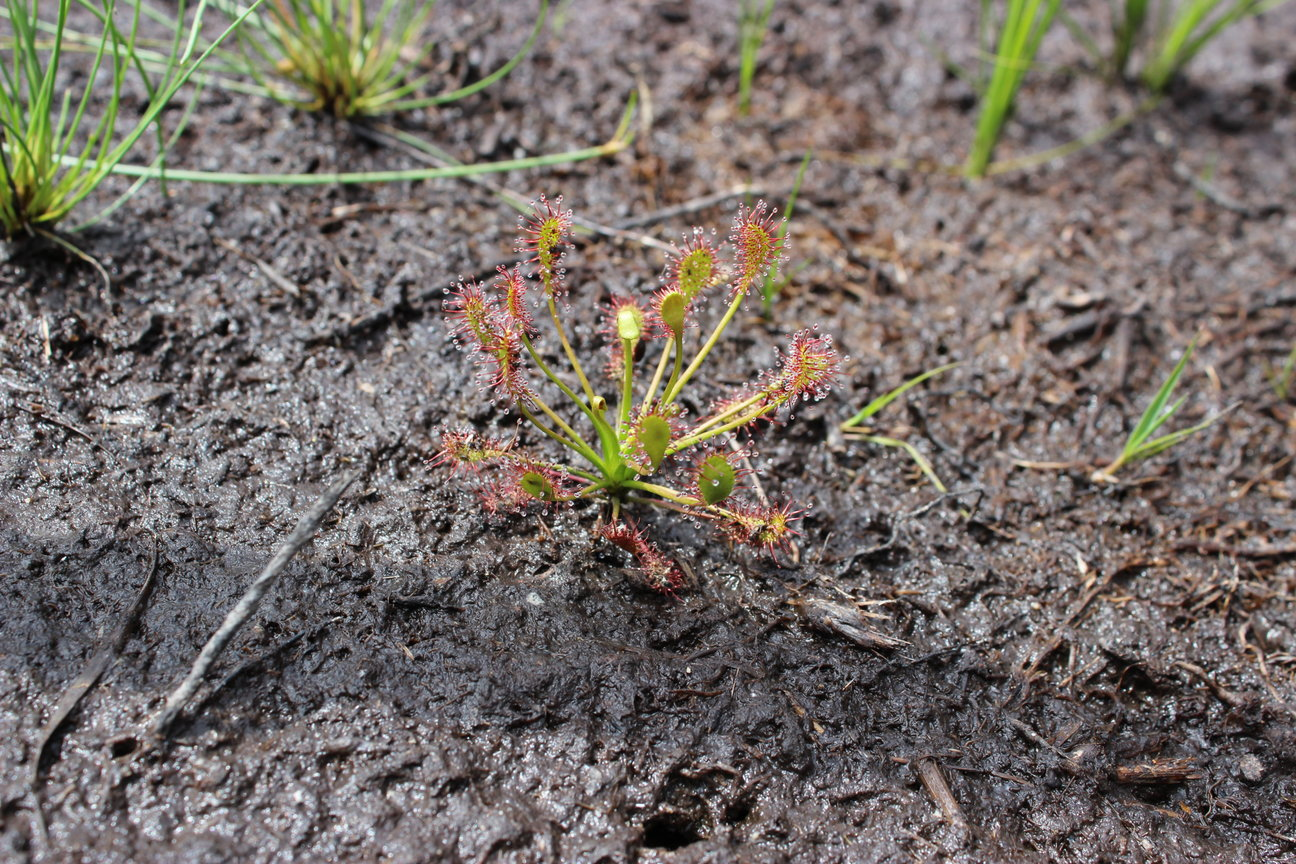
\includegraphics[trim=2.5cm 5cm 2.5cm 5cm, clip=true, width=\textwidth]{chap2/drosera_c.jpg}
        \caption{drosera}\label{fig:dro}
    \end{subfigure}
    \caption{Végétation présente sur le site de La Guette, et suivie lors des campagnes de mesure.}\label{fig:veg_other}
\end{figure}

\section{protocole végétation}
\label{sec:protocole_veg}


Le suivi non-destructif d'une végétation n'est pas triviale et nécessite la mise en place de protocoles particuliers en fonction du type de végétation.
L'objectif est de pouvoir estimer une biomasse produite en impactant au minimum la végétation en place.
Pour l'ensemble des espèces végétales présentes dans les embases servant à la mesure des flux un recouvrement à été estimé, à l’œil.


\subsubsection{La strate arbustive}
Pour la strate arbustive des mesures de hauteur moyenne ont été effectuées, en mesurant depuis le niveau du sol, ou le toit des sphaignes, si elles étaient présentes, jusqu'au sommet de l'individu.
\begin{figure}
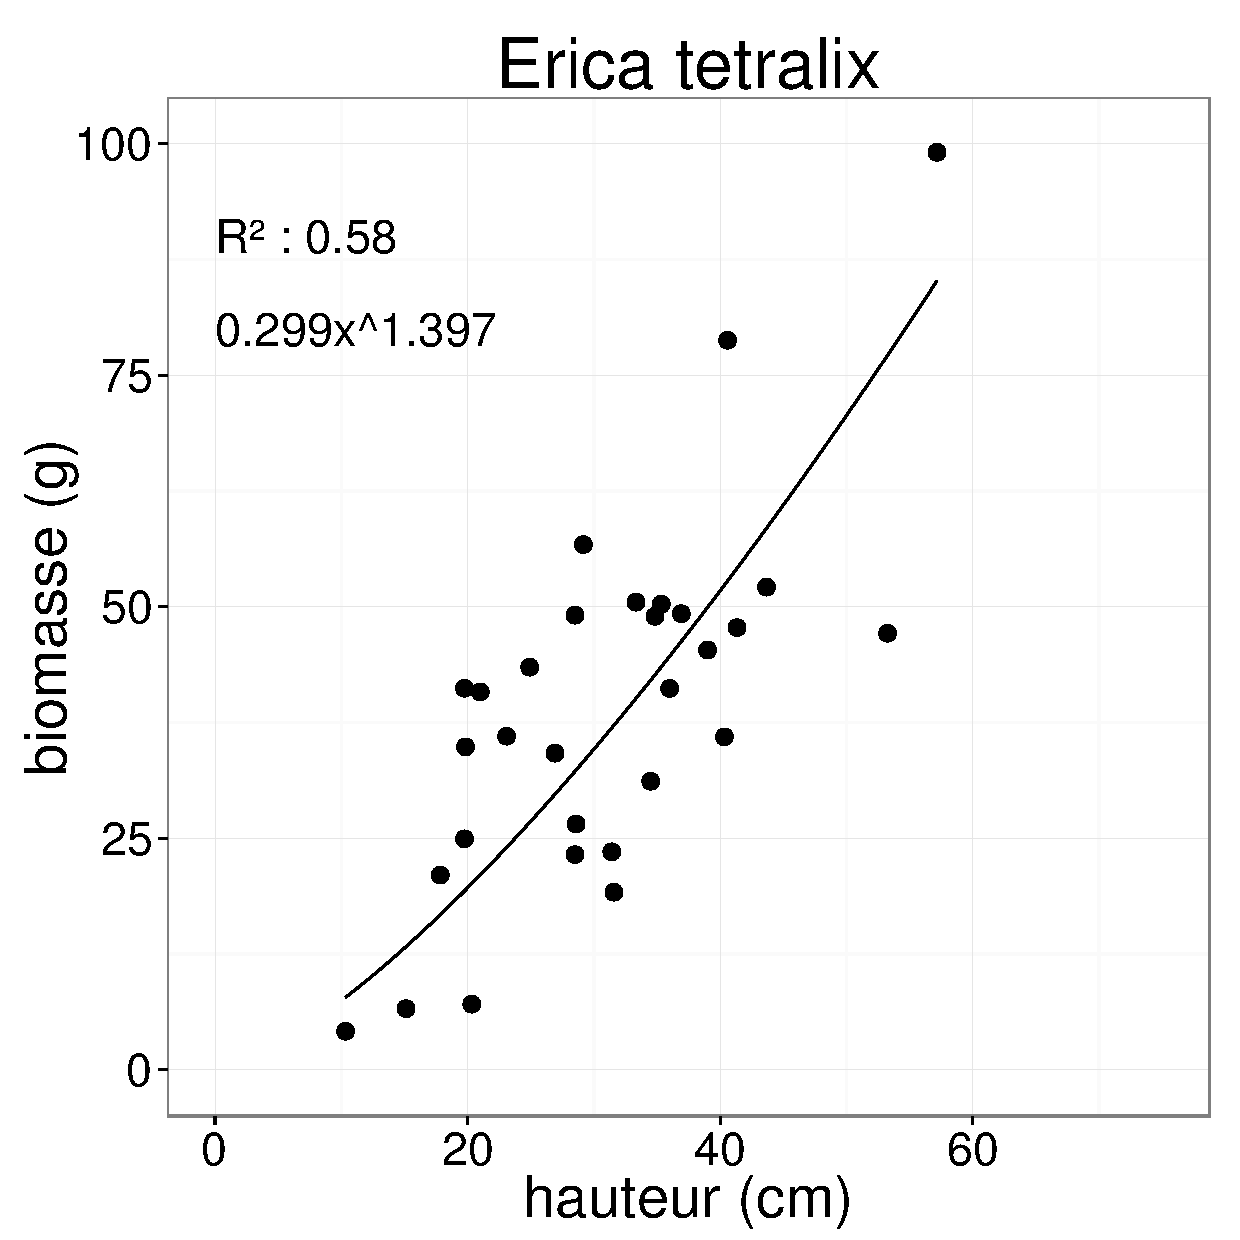
\includegraphics[width=.5\textwidth]{chap2/cal_tetra_eq}
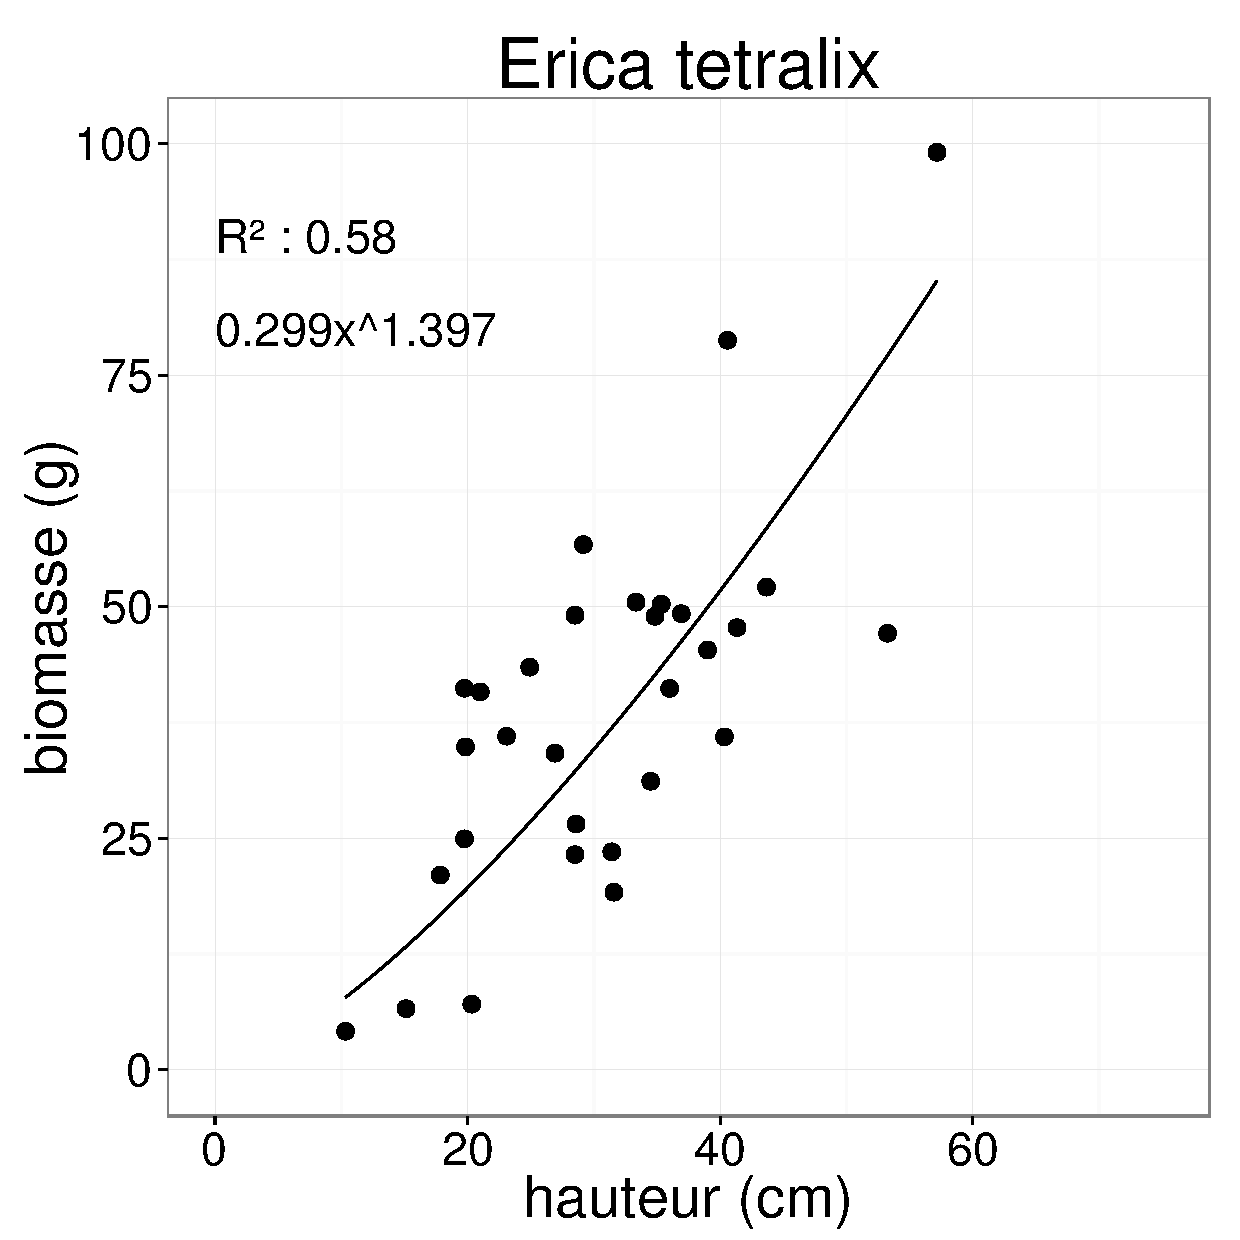
\includegraphics[width=.5\textwidth]{chap2/cal_tetra_eq}
\caption{Calibration de la biomasse en fonction de la hauteur}
\label{fig:cal_arbu}
\end{figure}

\subsubsection{La strate herbacée}
Pour la strate herbacée, en 2013, 5 individus des deux espèces majoritaires (Eriophorum vaginatum ? augustifolium ?, Molinia Caerulea) ont été marqués afin de pourvoir les mesurer plusieurs fois au cours de la saison.
Cependant les difficultés à retrouver les individus marqués couplés à la mort d'un nombre important d'entre eux n'ont pas permis d'acquérir de résultats significatifs.
En conséquence en 2014 ces deux espèces ont fait l'objet de comptage exhaustif et de mesure de hauteur moyenne.


\begin{figure}
	\centering
	\begin{subfigure}[t]{0.5\textwidth}
		\centering
		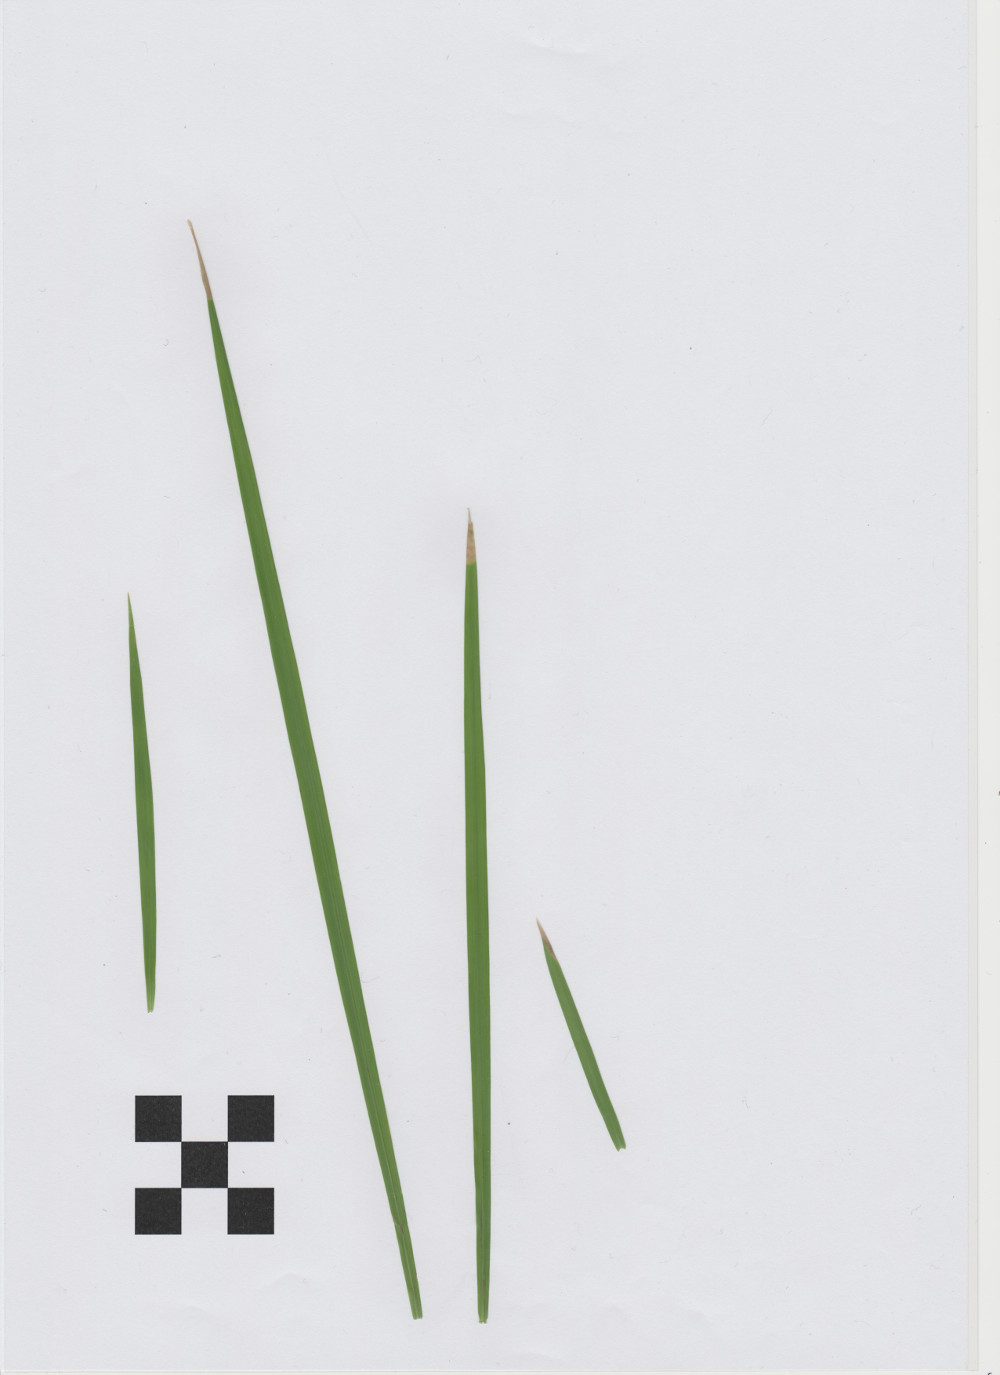
\includegraphics[width=.8\textwidth, frame]{chap2/Cch_moli_A_1to4}
		\caption{image scannée}
	\end{subfigure}%
	\begin{subfigure}[t]{0.5\textwidth}
		\centering
		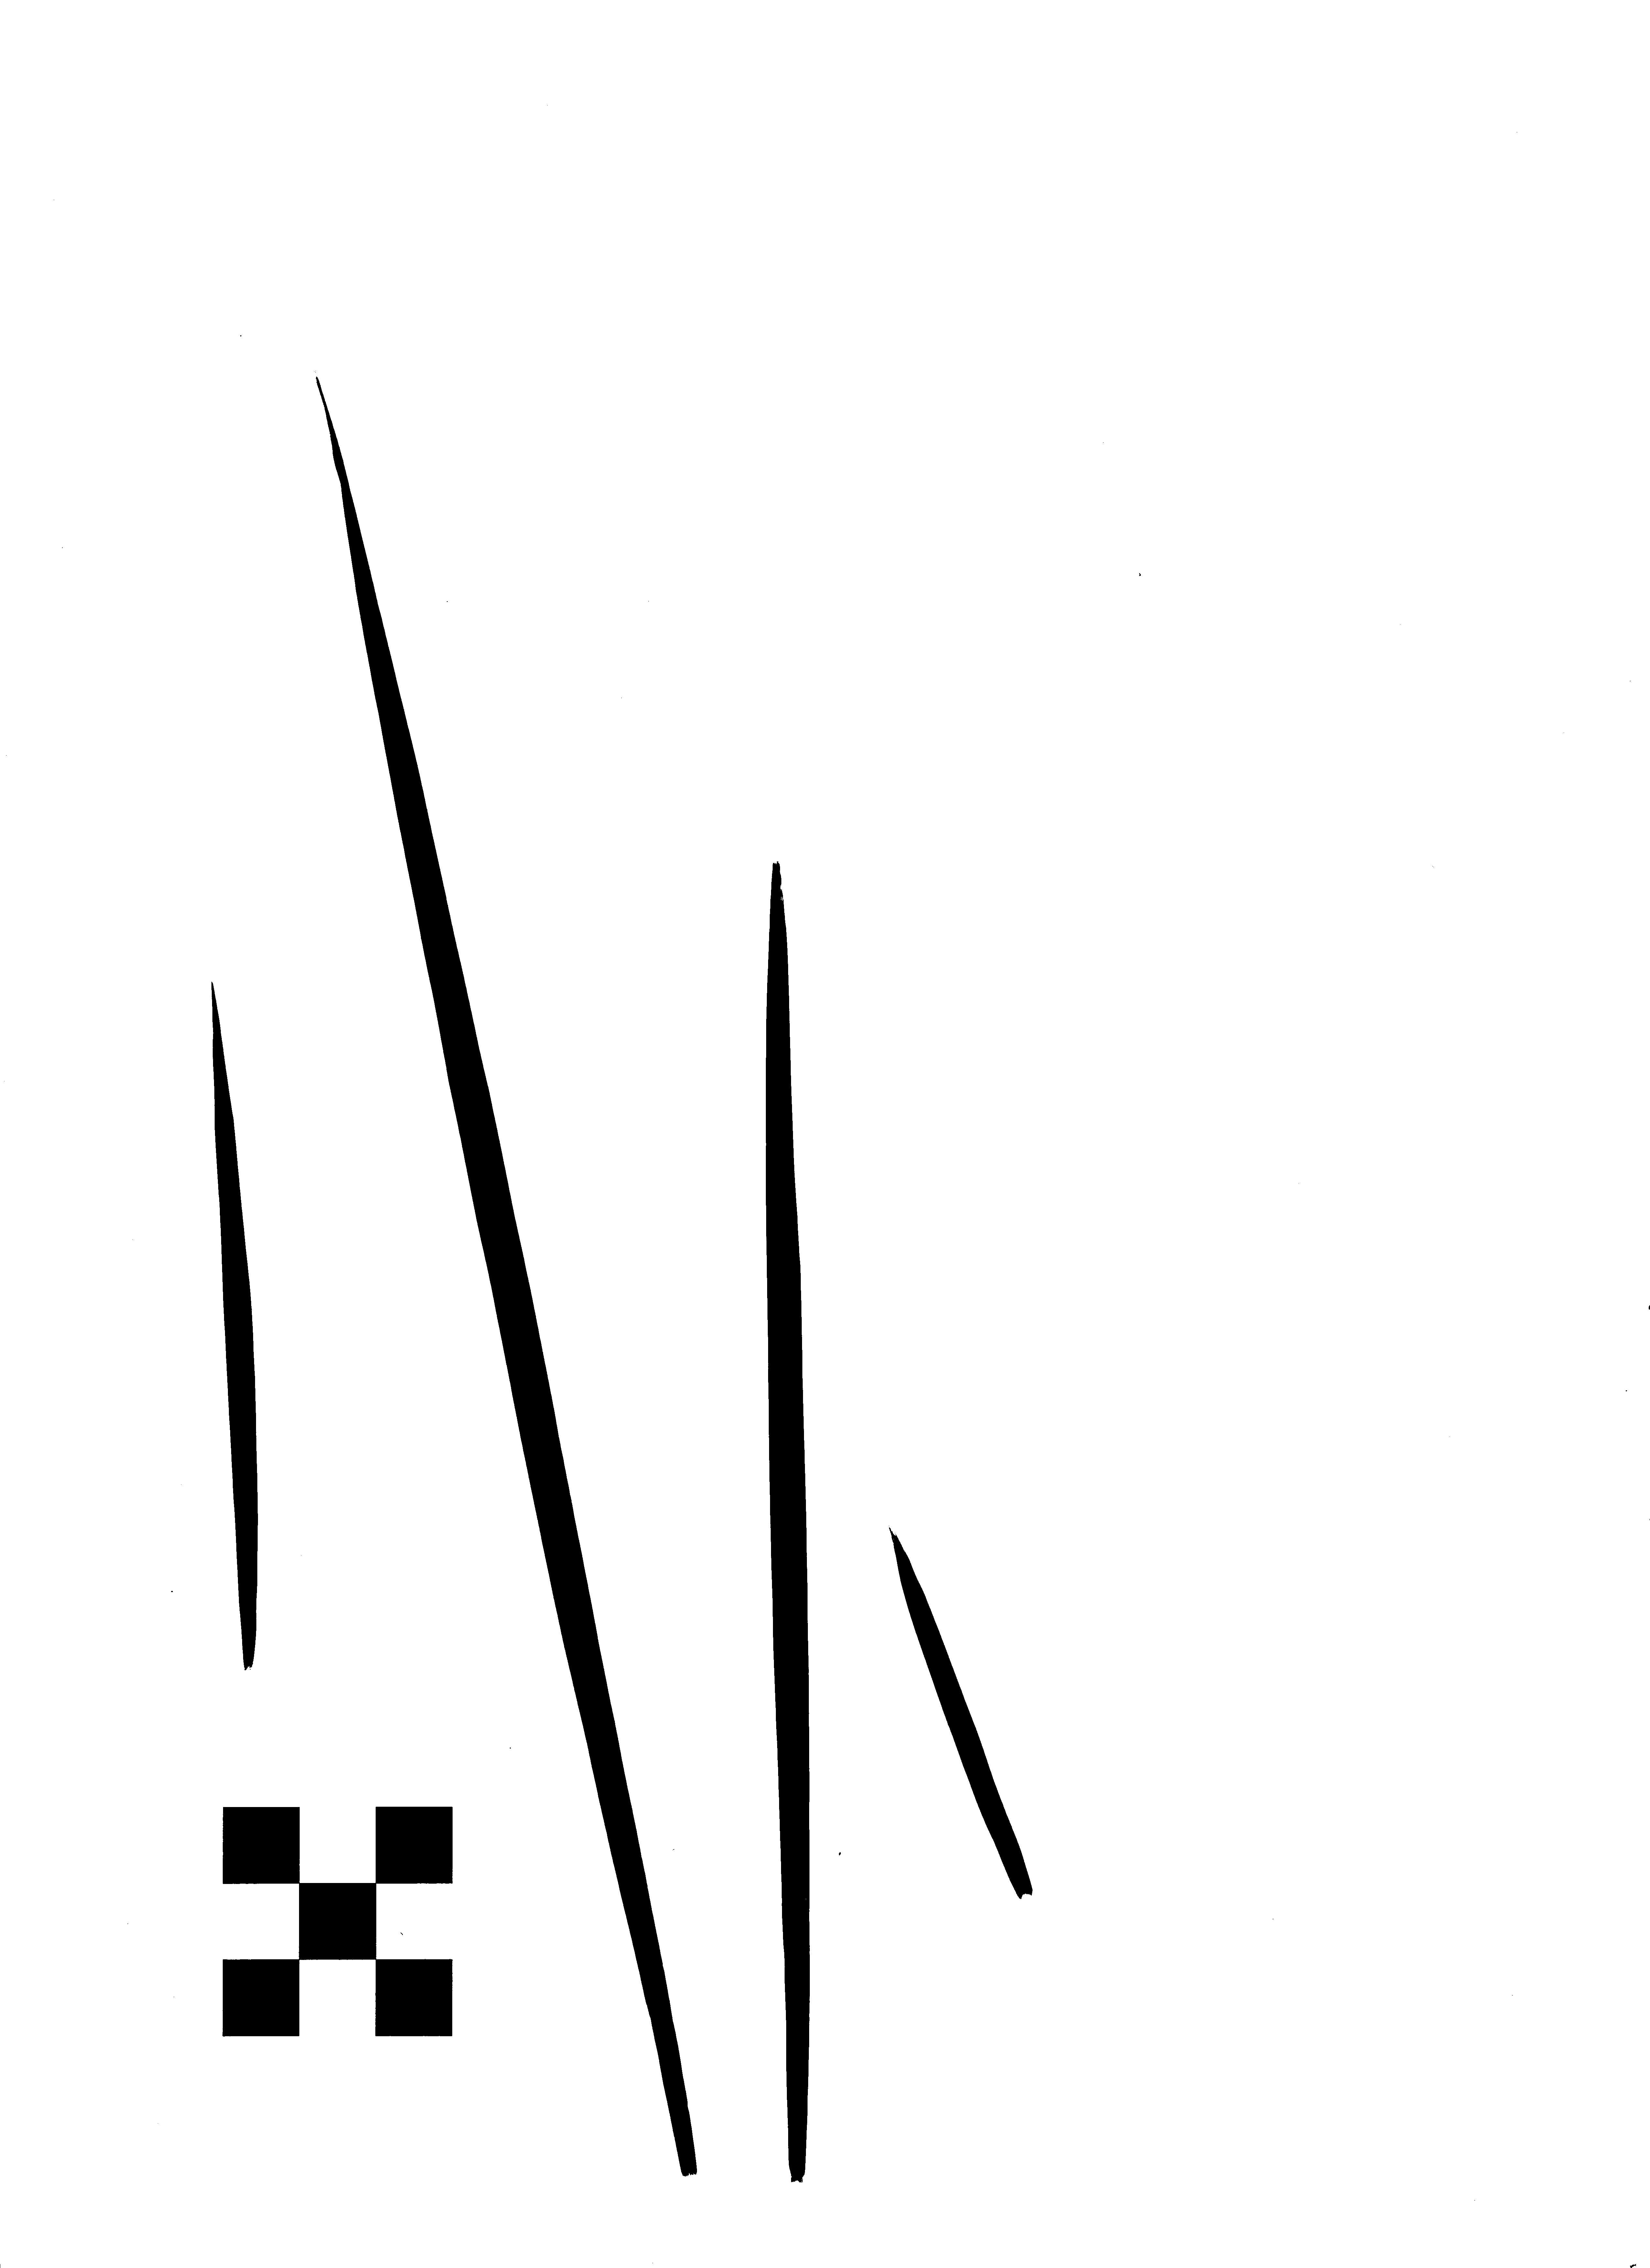
\includegraphics[width=.8\textwidth, frame]{chap2/Cch_moli_A_1to4_mod}
		\caption{image binarisée}
	\end{subfigure}
%    \caption{Caption place holder}
\caption{Scanne des feuilles}
\label{fig:scan_mol}
\end{figure}


\begin{figure}
	\centering
	\begin{subfigure}[t]{0.5\textwidth}
		\centering
		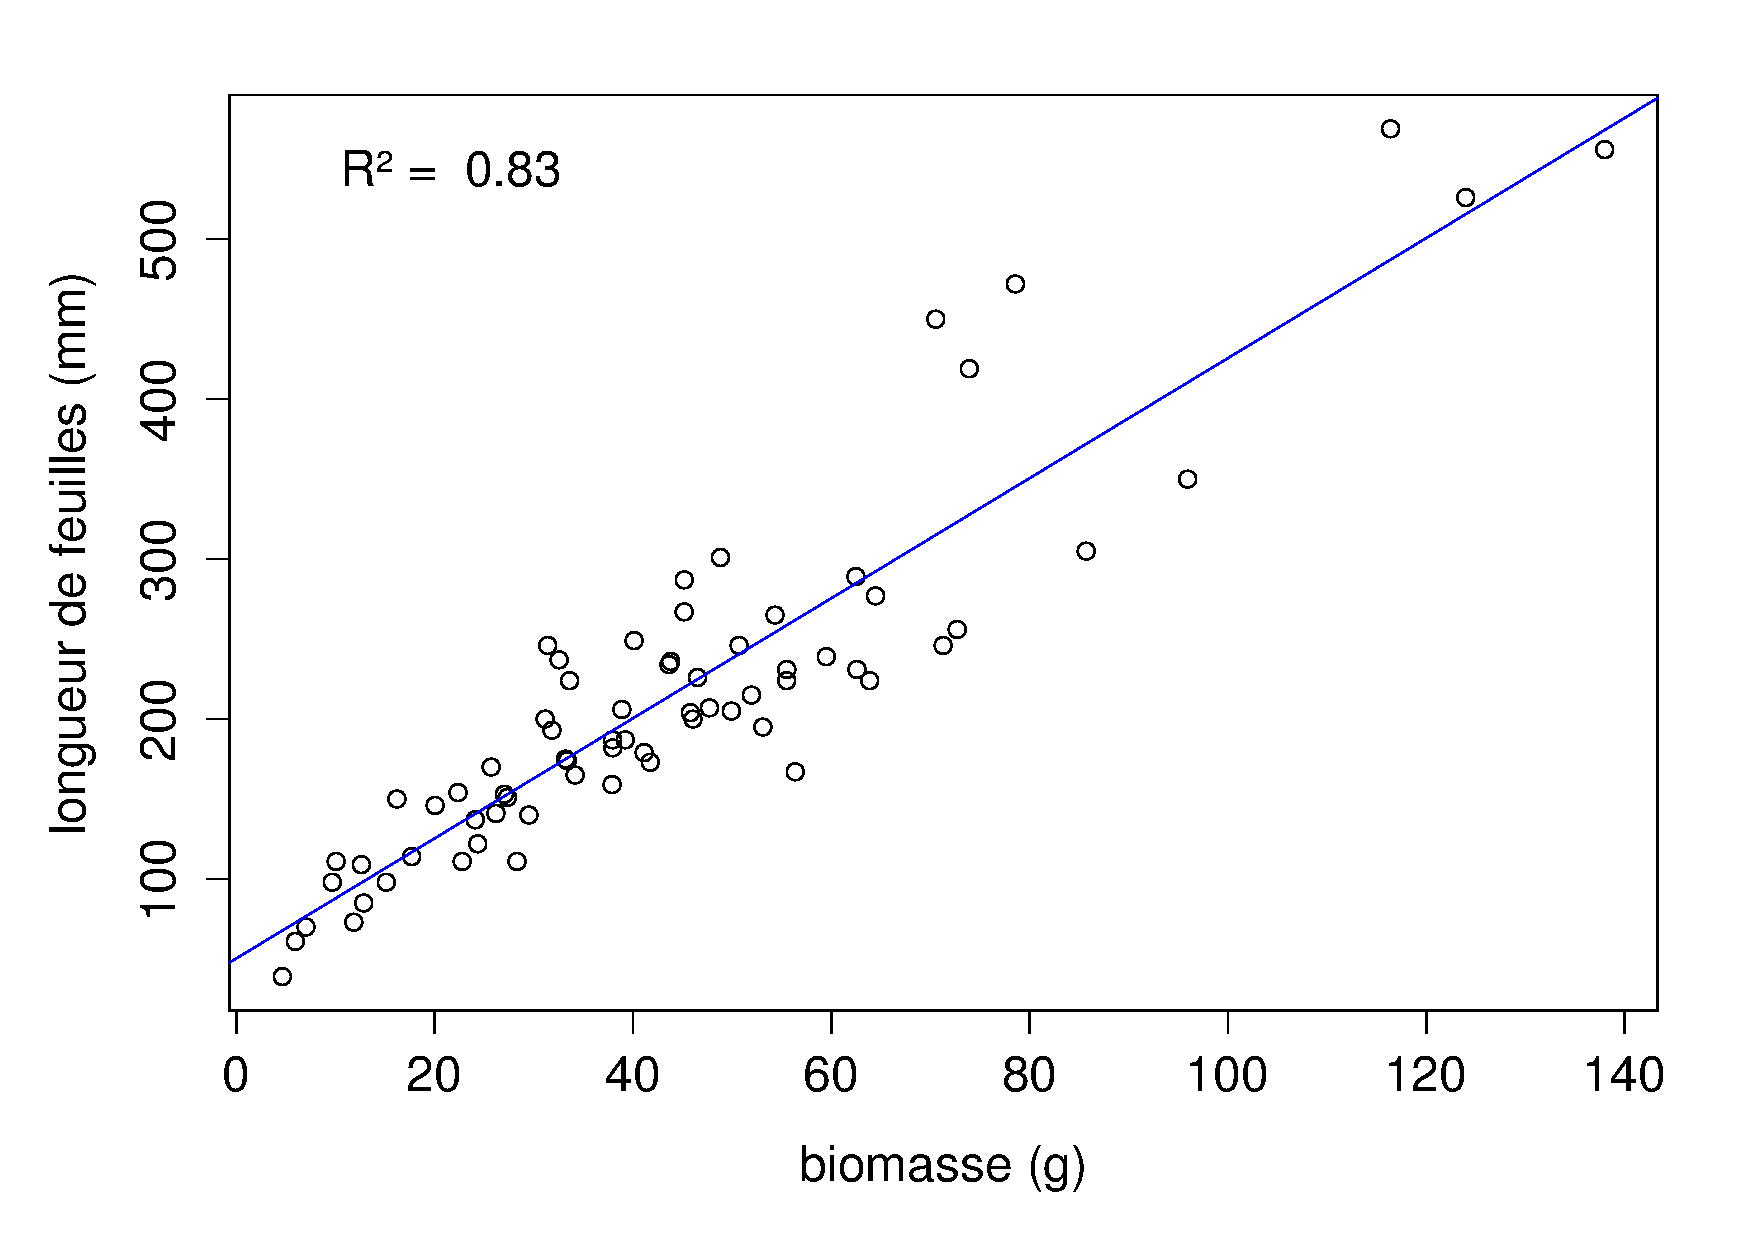
\includegraphics[width=\textwidth]{chap2/mol_lon_bioM}
		\caption{Molinia caerulea -- biomasse}
	\end{subfigure}%
	\begin{subfigure}[t]{0.5\textwidth}
		\centering
		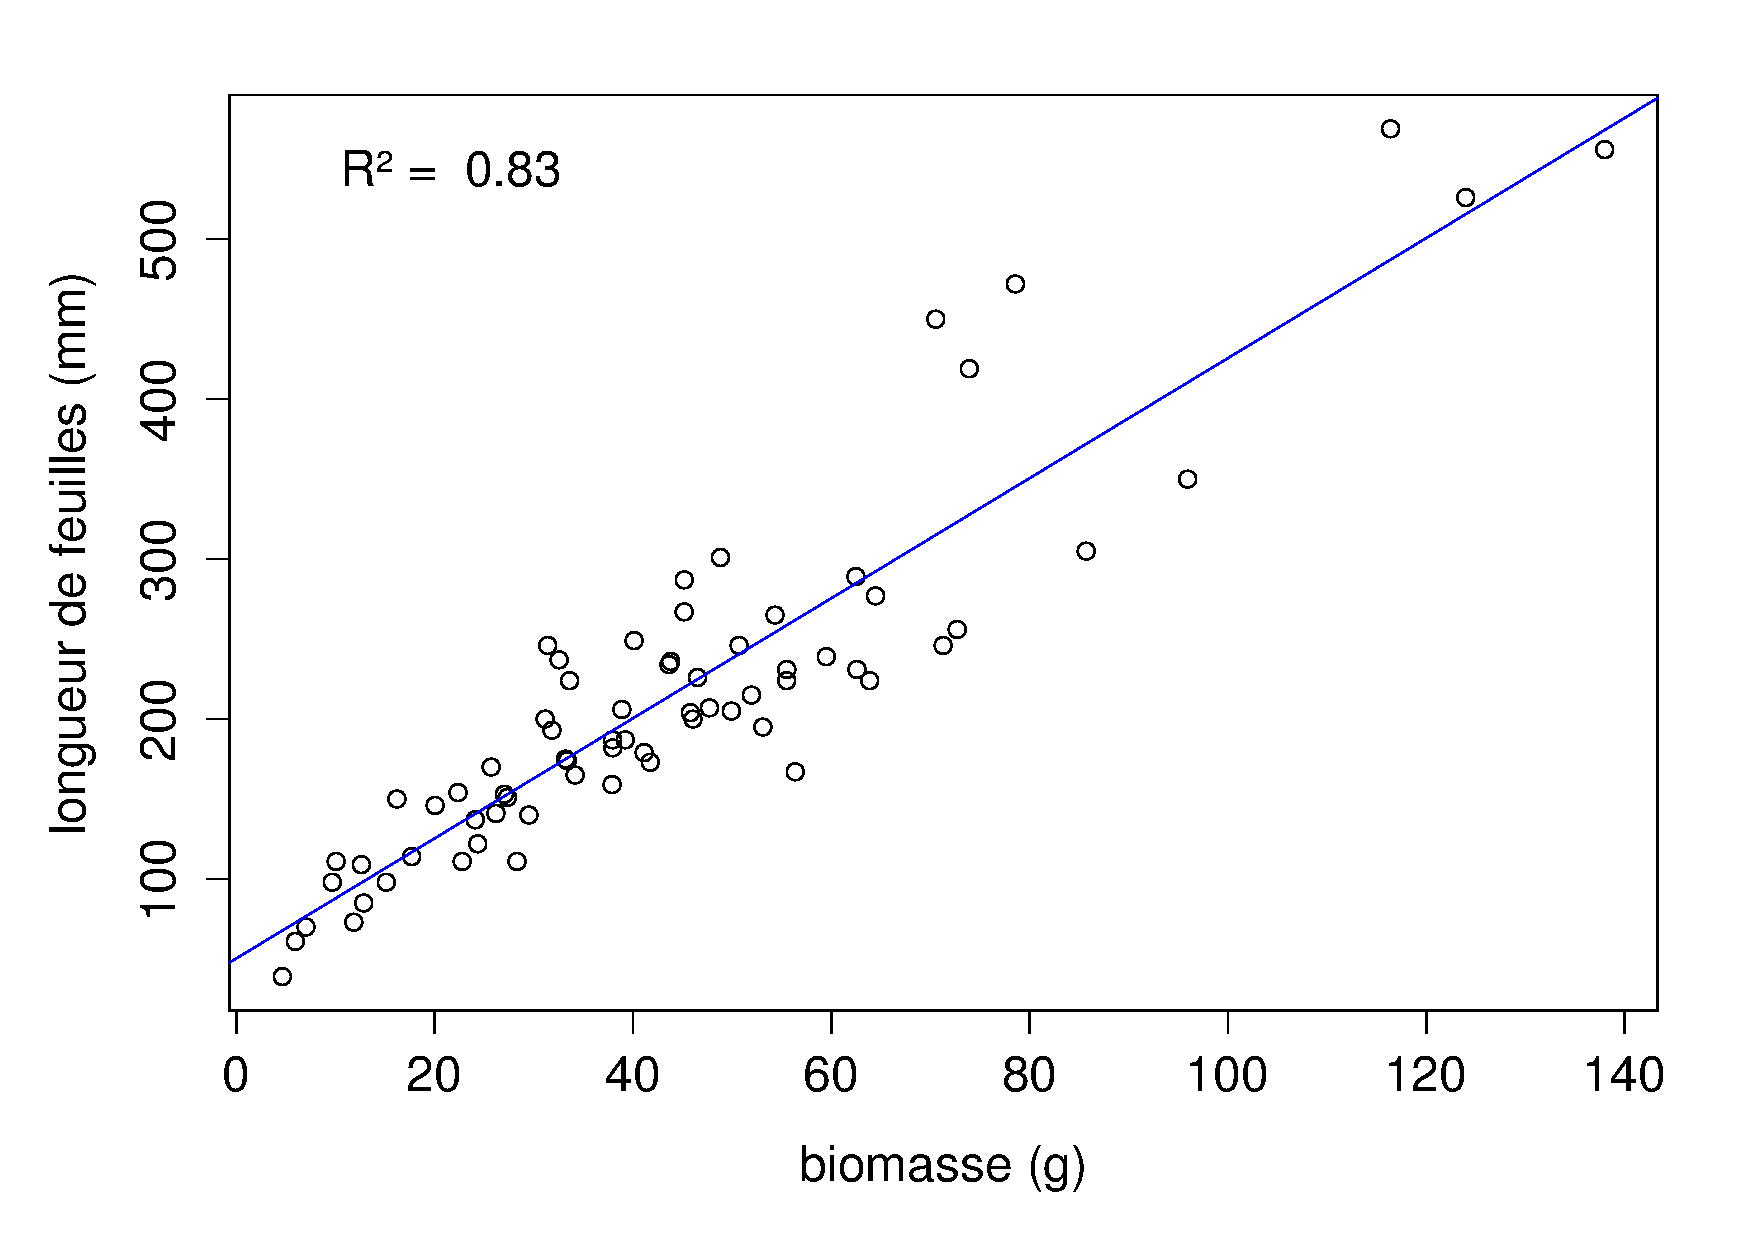
\includegraphics[width=\textwidth]{chap2/mol_lon_bioM}
		\caption{Eriophorum -- biomasse}
	\end{subfigure}
	
	
	\begin{subfigure}[t]{0.5\textwidth}
		\centering
		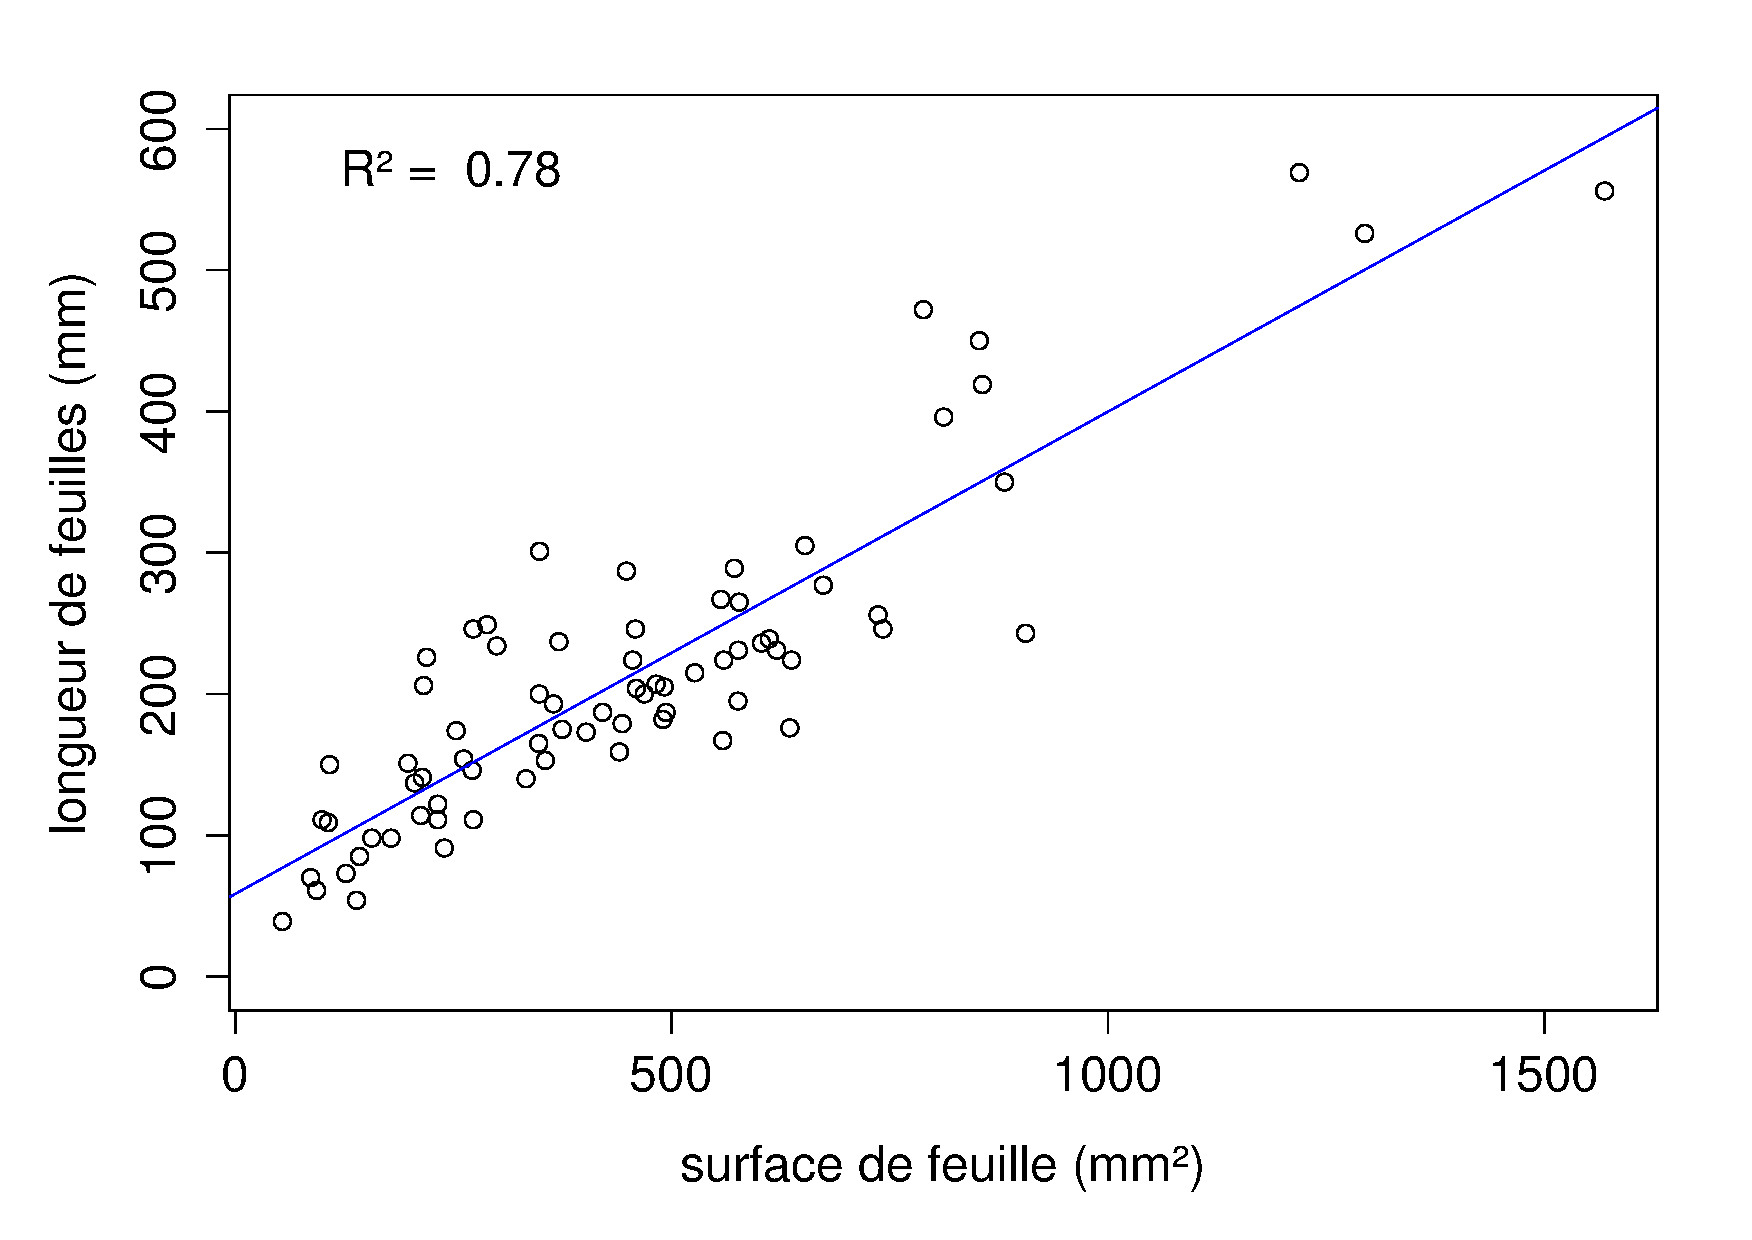
\includegraphics[width=\textwidth]{chap2/mol_lon_surf}
		\caption{Molinia caerulea -- surface}
	\end{subfigure}%
	\begin{subfigure}[t]{0.5\textwidth}
		\centering
		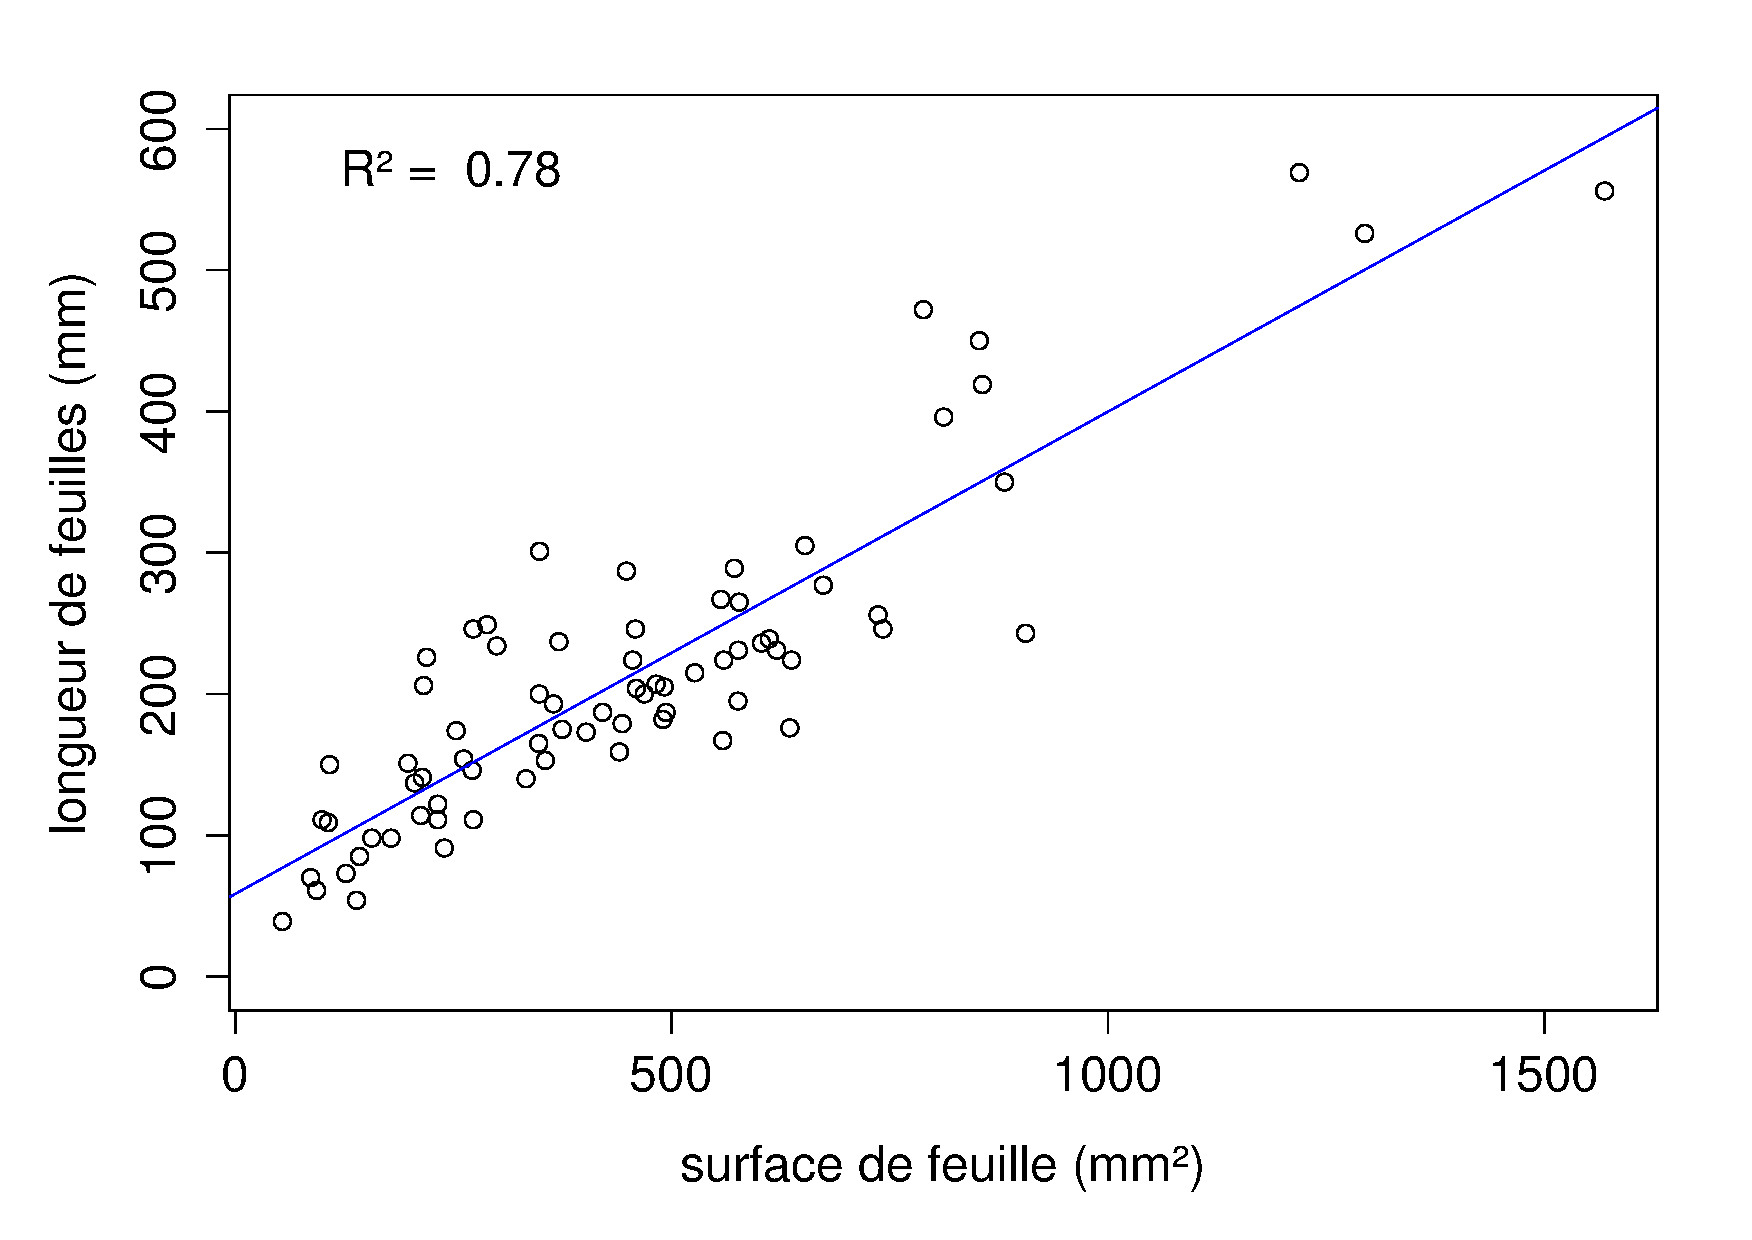
\includegraphics[width=\textwidth]{chap2/mol_lon_surf}
		\caption{Eriphorum -- surface}
	\end{subfigure}
%    \caption{Caption place holder}
\caption{Calibration de la biomasse herbacées pour \textit{molinia Caerulea} (a), pour \textit{eriophorum} (b) et de la surface de feuille pour \textit{molinia Caerulea} (c), pour \textit{eriophorum} (d) en fonction de la hauteur}
\label{fig:cal_herb}
\end{figure}




\section{package m70r}
\label{sec:pckg_m70r}

\begin{figure}
\centering
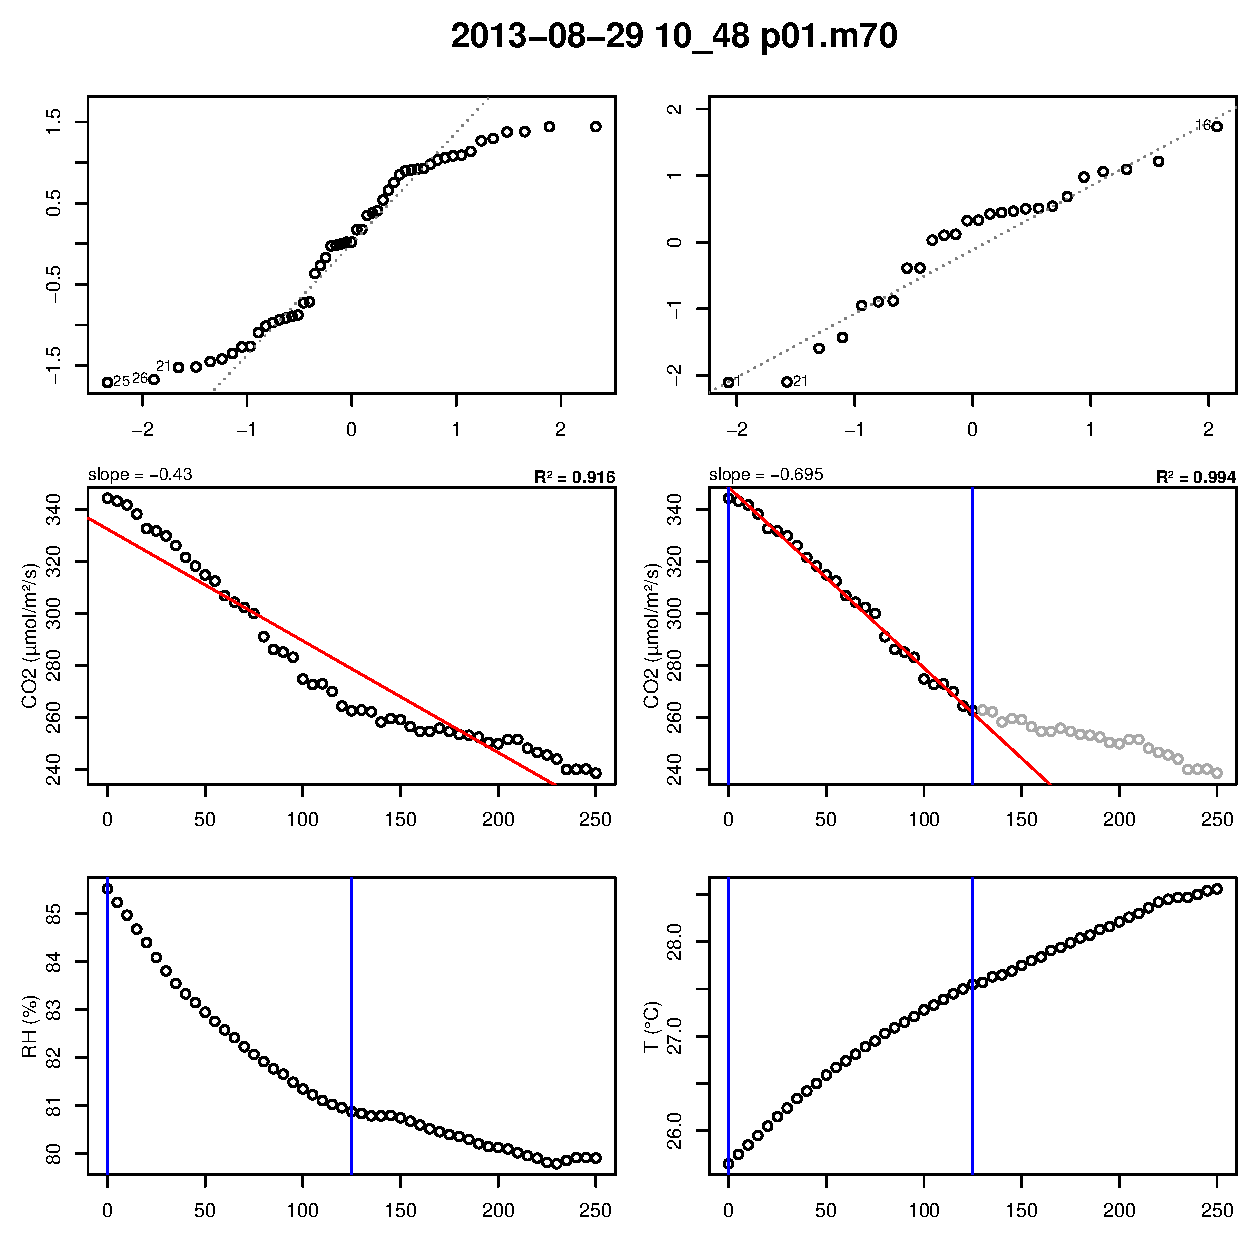
\includegraphics[width=.8\textwidth, frame]{annexes/m70r_diagplot}
\caption{Planche de graphes permettant le diagnostique des mesures de flux de \coo}
\label{fig:m70r_diagplot}
\end{figure}

Ce package contient une série de fonctions à utiliser avec le language R et qui permettent de traiter les fichiers *.m70 issue des sondes Vaisala.

\begin{itemize}
\item Générer des planches de graphes pour diagnostiquer les flux (Figure~\ref{fig:m70r_diagplot})
\item De comparer l'effet du retrait de certains points. La figure~\ref{fig:m70r_diagplot} montre ainsi une mesure pour laquelle l'assimilation de \coo par photosynthèse est tellement forte qu'elle semble être stoppée abruptement au delà d'un certain seuil.
\item De conserver les changements effectués dans un fichier séparé du fichier source, qui reste donc intact.
\item De calculer les flux net.
\end{itemize}

\clearpage
\section{Résultats des ACP}
\label{sec:acp}

Les données de \chh étant moins nombreuses que les données de \coo, deux ACP ont été effectuées, l'une sans les données de \chh et l'autre avec, afin de maximiser le nombre d'observation utilisés.

\subsection{ACP des flux de \coo et des facteurs contrôlants (sans \chh)}

\begin{figure}[!hbt]
\centering
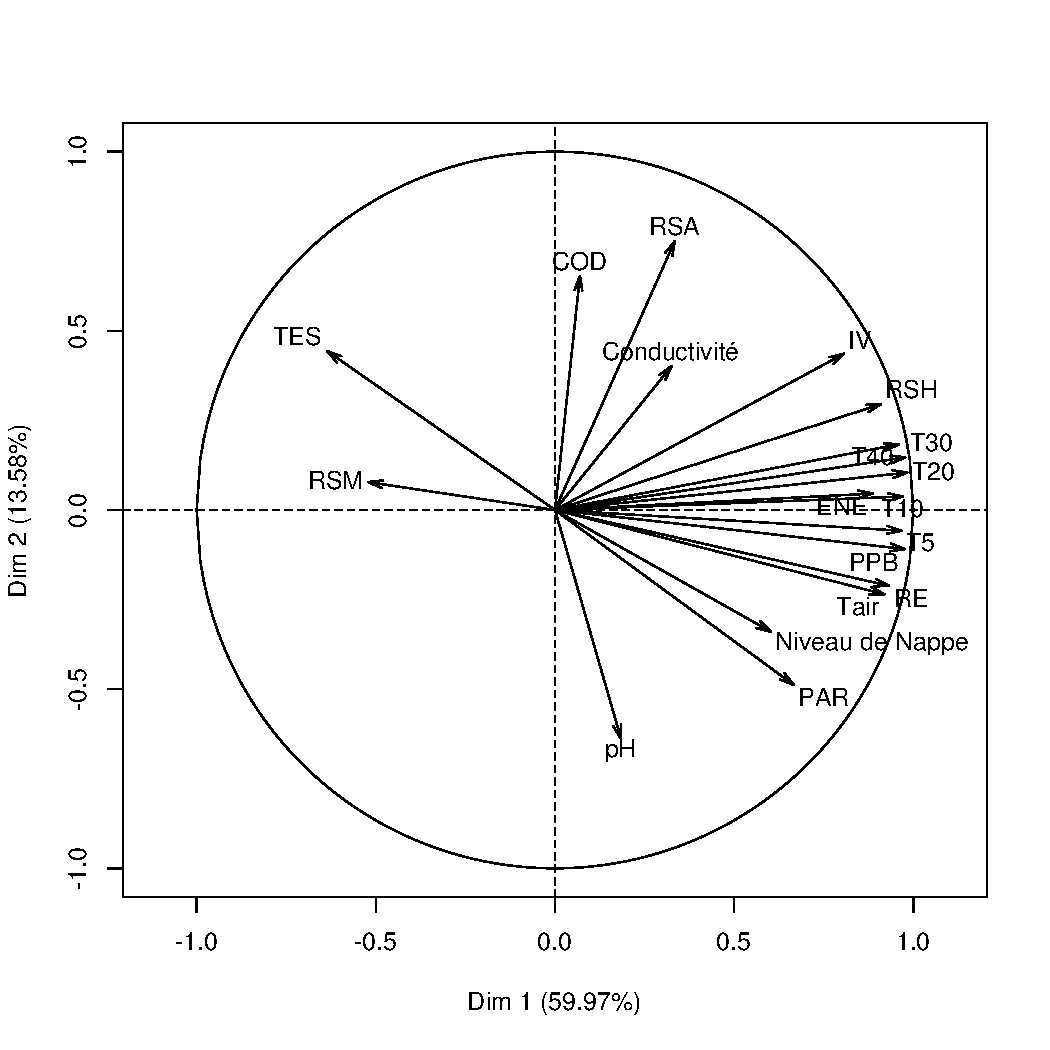
\includegraphics[width=.8\textwidth]{annexes/acp_co2_var_12}\\
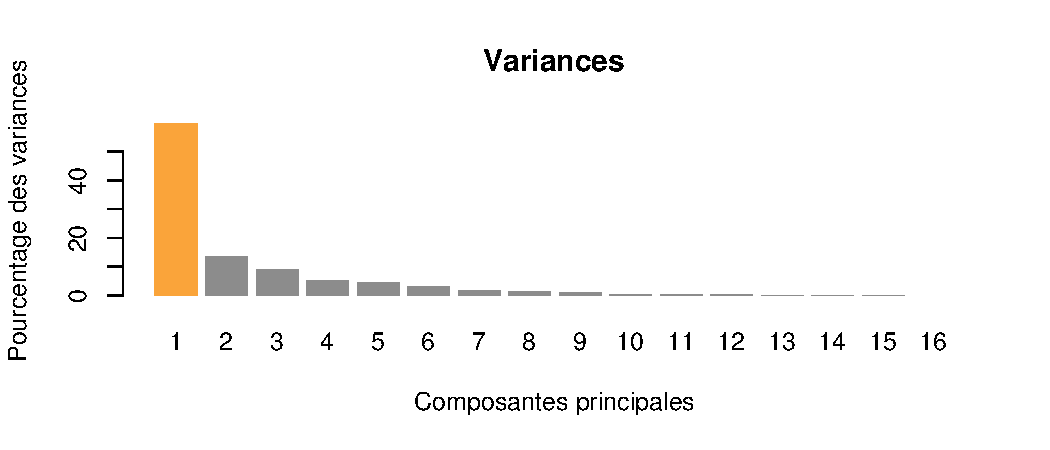
\includegraphics[width=.8\textwidth]{annexes/acp_co2_hist}
\caption{Dimension 1 et 2 de l'ACP sans les données de \chh (en haut), et pourcentage de variance expliqué par dimension (en bas)}
\label{fig:acp_co2}
\end{figure}


\subsection{ACP des flux et des facteurs contrôlants (avec \chh)}

\begin{figure}[!hbt]
\centering
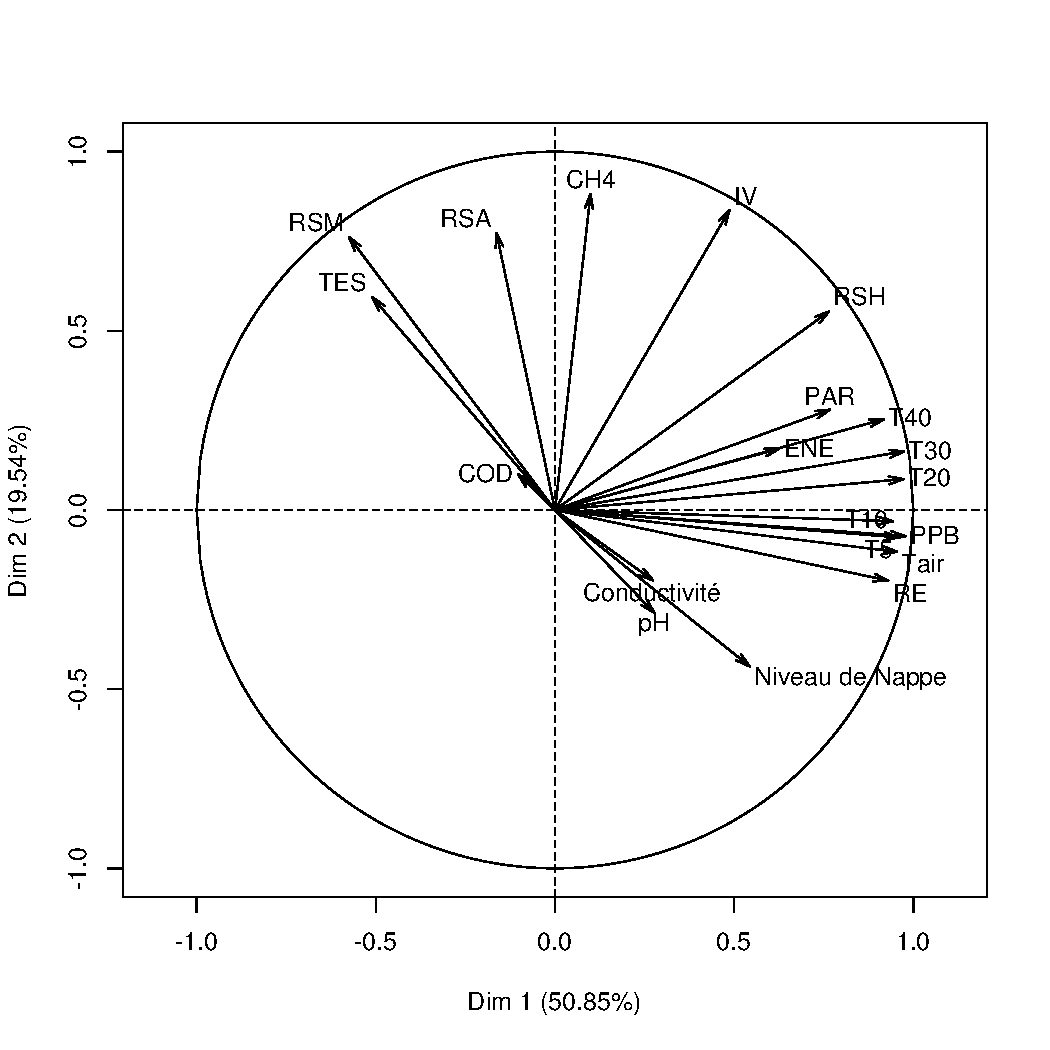
\includegraphics[width=.8\textwidth]{annexes/acp_ch4_var_12}\\
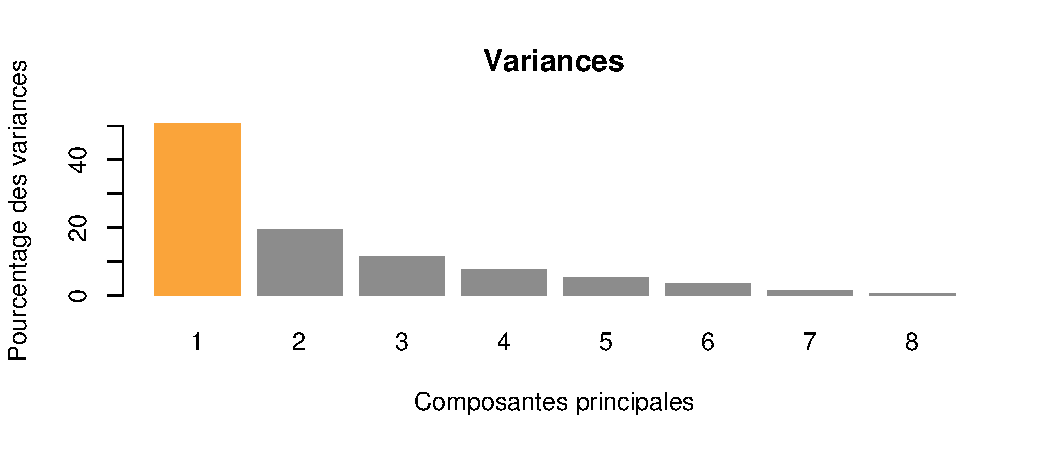
\includegraphics[width=.8\textwidth]{annexes/acp_ch4_hist}
\caption{Dimension 1 et 2 de l'ACP avec les données de \chh (en haut), et pourcentage de variance expliqué par dimension (en bas)}
\label{fig:acp_ch4}
\end{figure}


\section{Le projet \textsc{carbiodiv}}
\label{sec:carbiodiv}

Ce projet vise à restaurer l'hydrologie de la tourbière de La Guette et de suivre les effets de cette restauration sur les flux de carbone et la biodiversité.
Ce projet implique donc des laboratoires scientifiques (ISTO, LPC2E) une cellule de recherche et développement de l'Université d'Orléans (CETRAHE), des associations (SNE, CERCOPE, LIN'Eco), et une entreprise (Environnement41).

Carte Nécessaire.



\section{Calibrations flux de GES et facteurs contrôlant}
\label{sec:calib_flux}

\begin{figure}[!hbt]
\centering
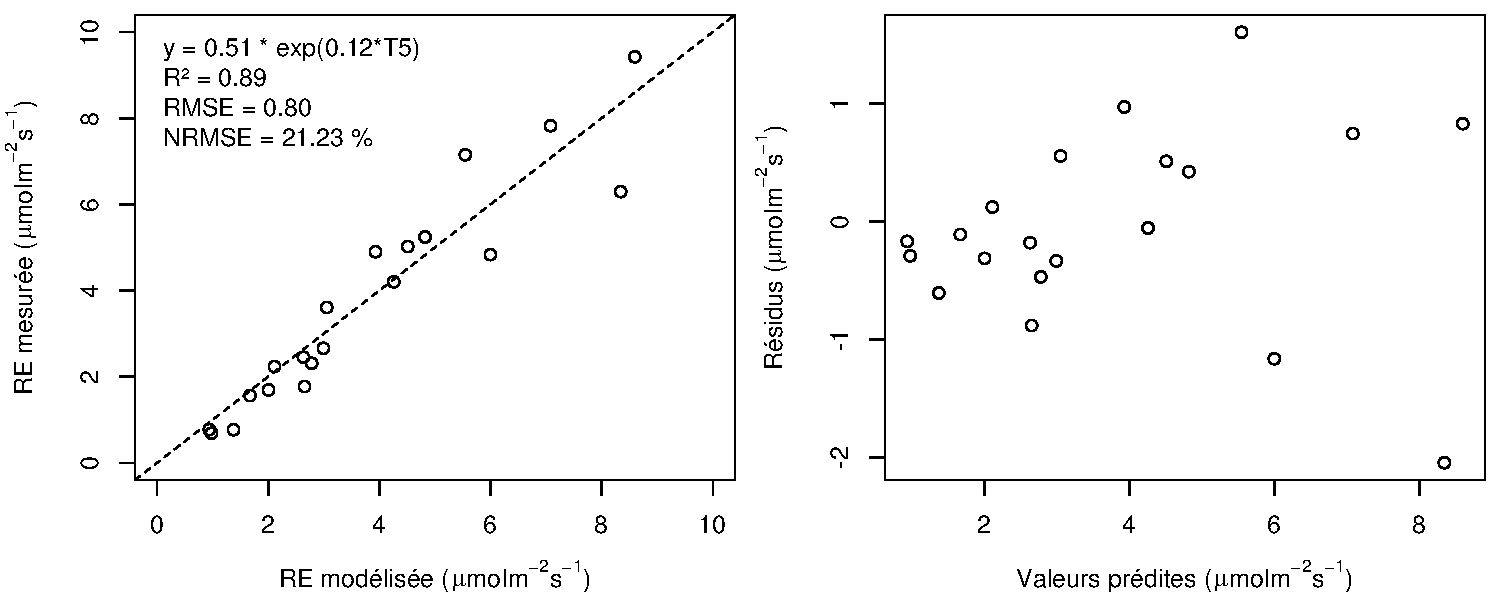
\includegraphics[width=.8\textwidth]{annexes/ER_T5_mdl_mesmod}\\
\caption{Résultat de la calibration de la RE avec un modèle exponentiel et en utilisant la température à \SI{-5}{\centi\metre}. À gauche la relation entre la RE mesurée et la RE modélisée et à gauche la distribution des résidus.}
\label{fig:RE_T5}
\end{figure}




\clearpage
\section{Cartes des flux par placettes}
\label{sec:carte_flux}

\subsection{PPB}
\label{subsec:carte_ppb}
La calibration des placettes p05, p13 et p15 n'a pas convergée.

\begin{figure}[!hbt]
\centering
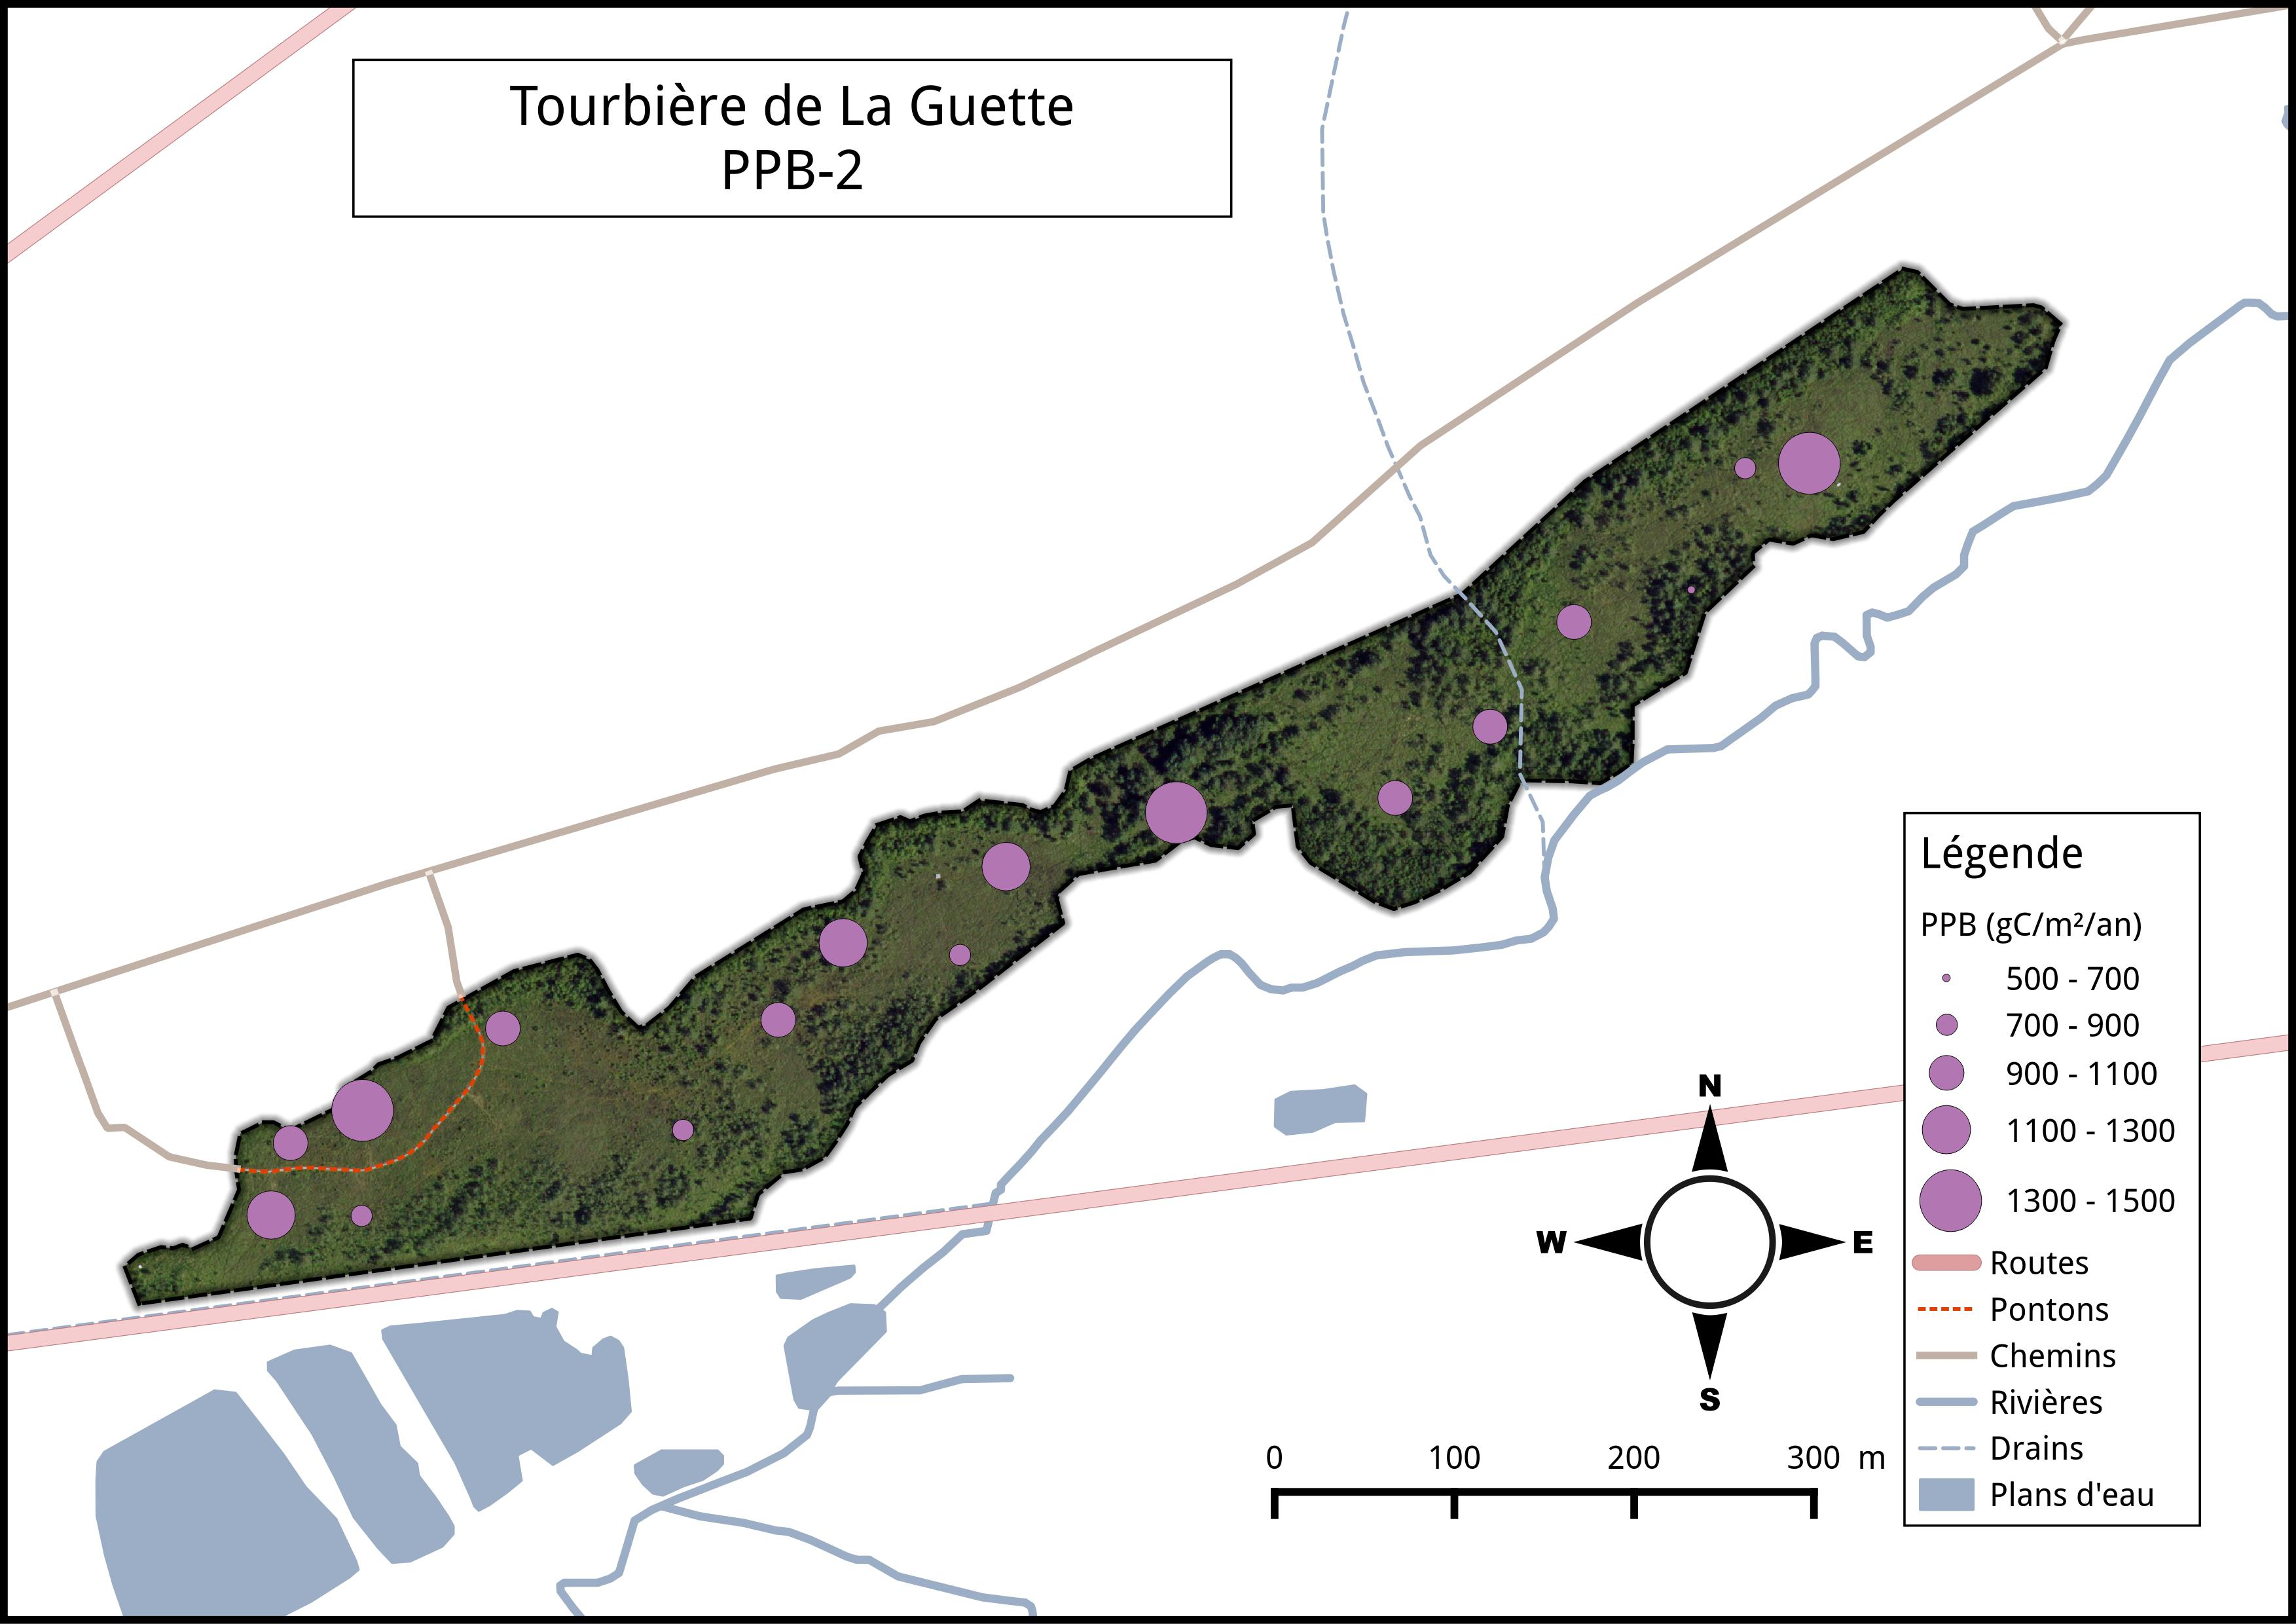
\includegraphics[width=.9\textwidth]{annexes/carte_PPB-2}
\caption{Répartition de RE sur la tourbière de La Guette en \si{\gcma} à partir du modèle PPB-2}
\label{fig:rep_PPB-2}
\end{figure}

\clearpage
\subsection{RE}
\label{subsec:carte_re}

\begin{figure}[!hbt]
\centering
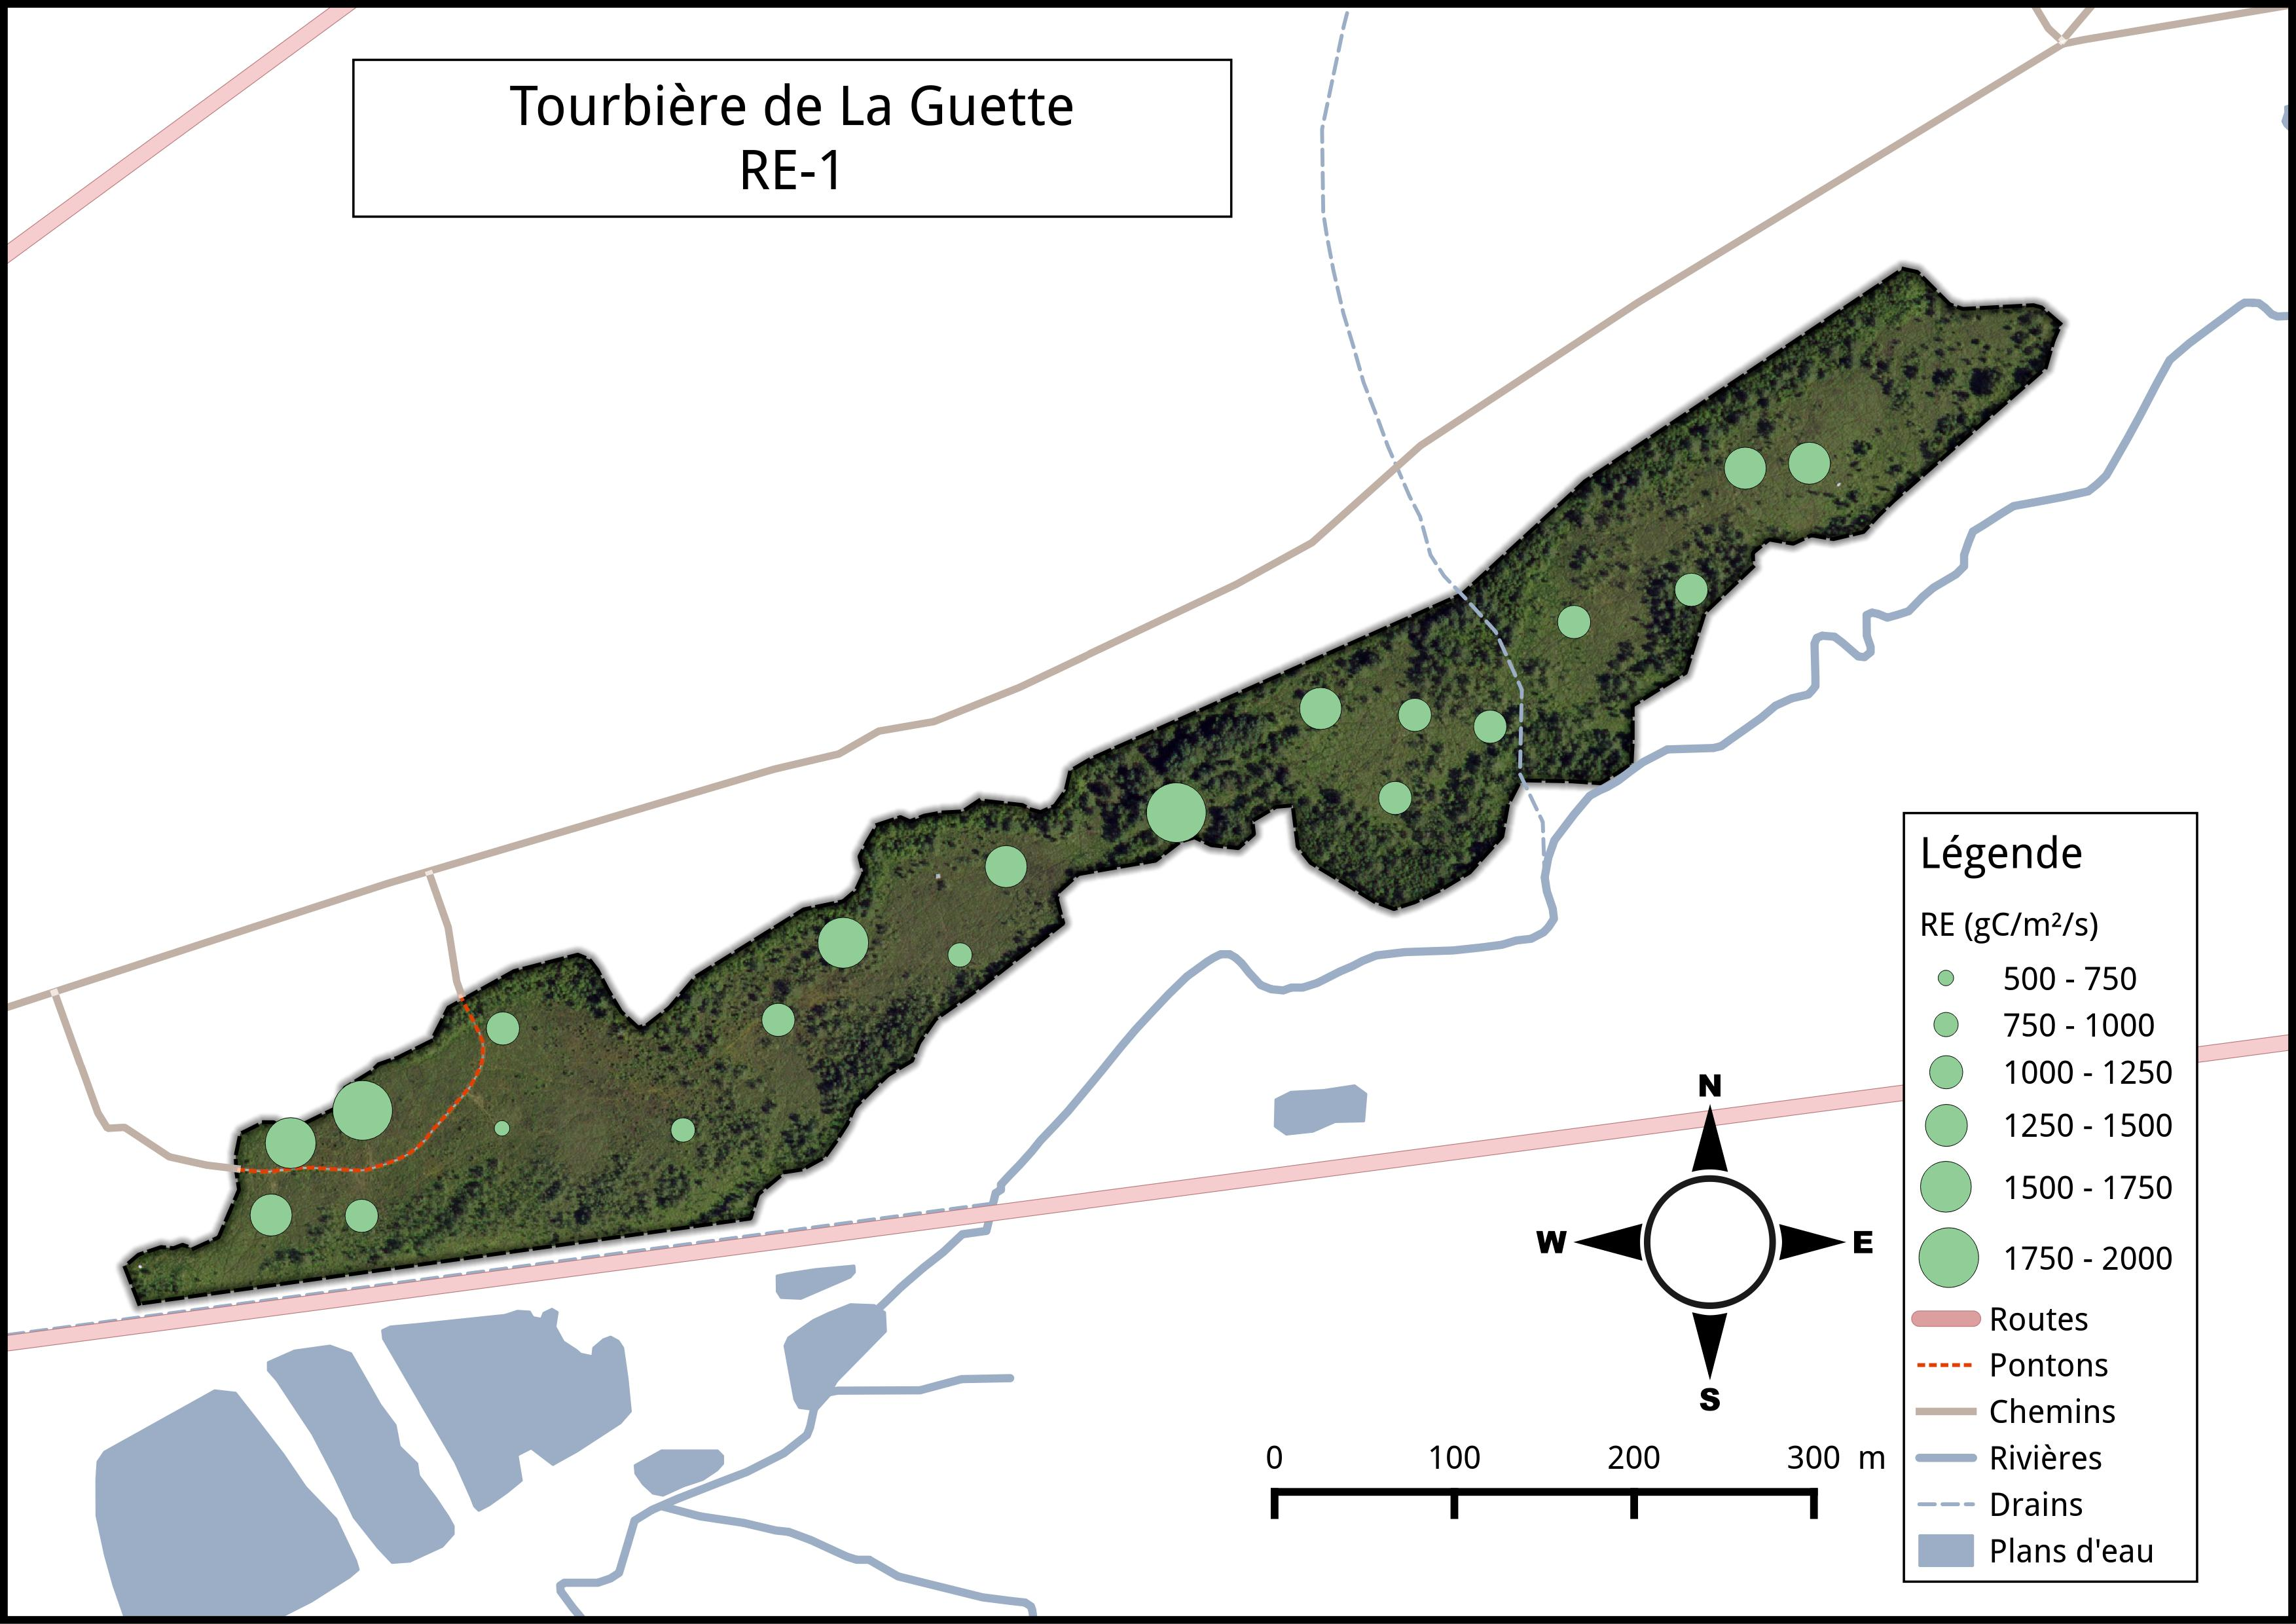
\includegraphics[width=.9\textwidth]{annexes/carte_RE-1}\\
\caption{Répartition de RE sur la tourbière de La Guette en \si{\gcma} à partir du modèle RE-1}
\label{fig:rep_RE-1}
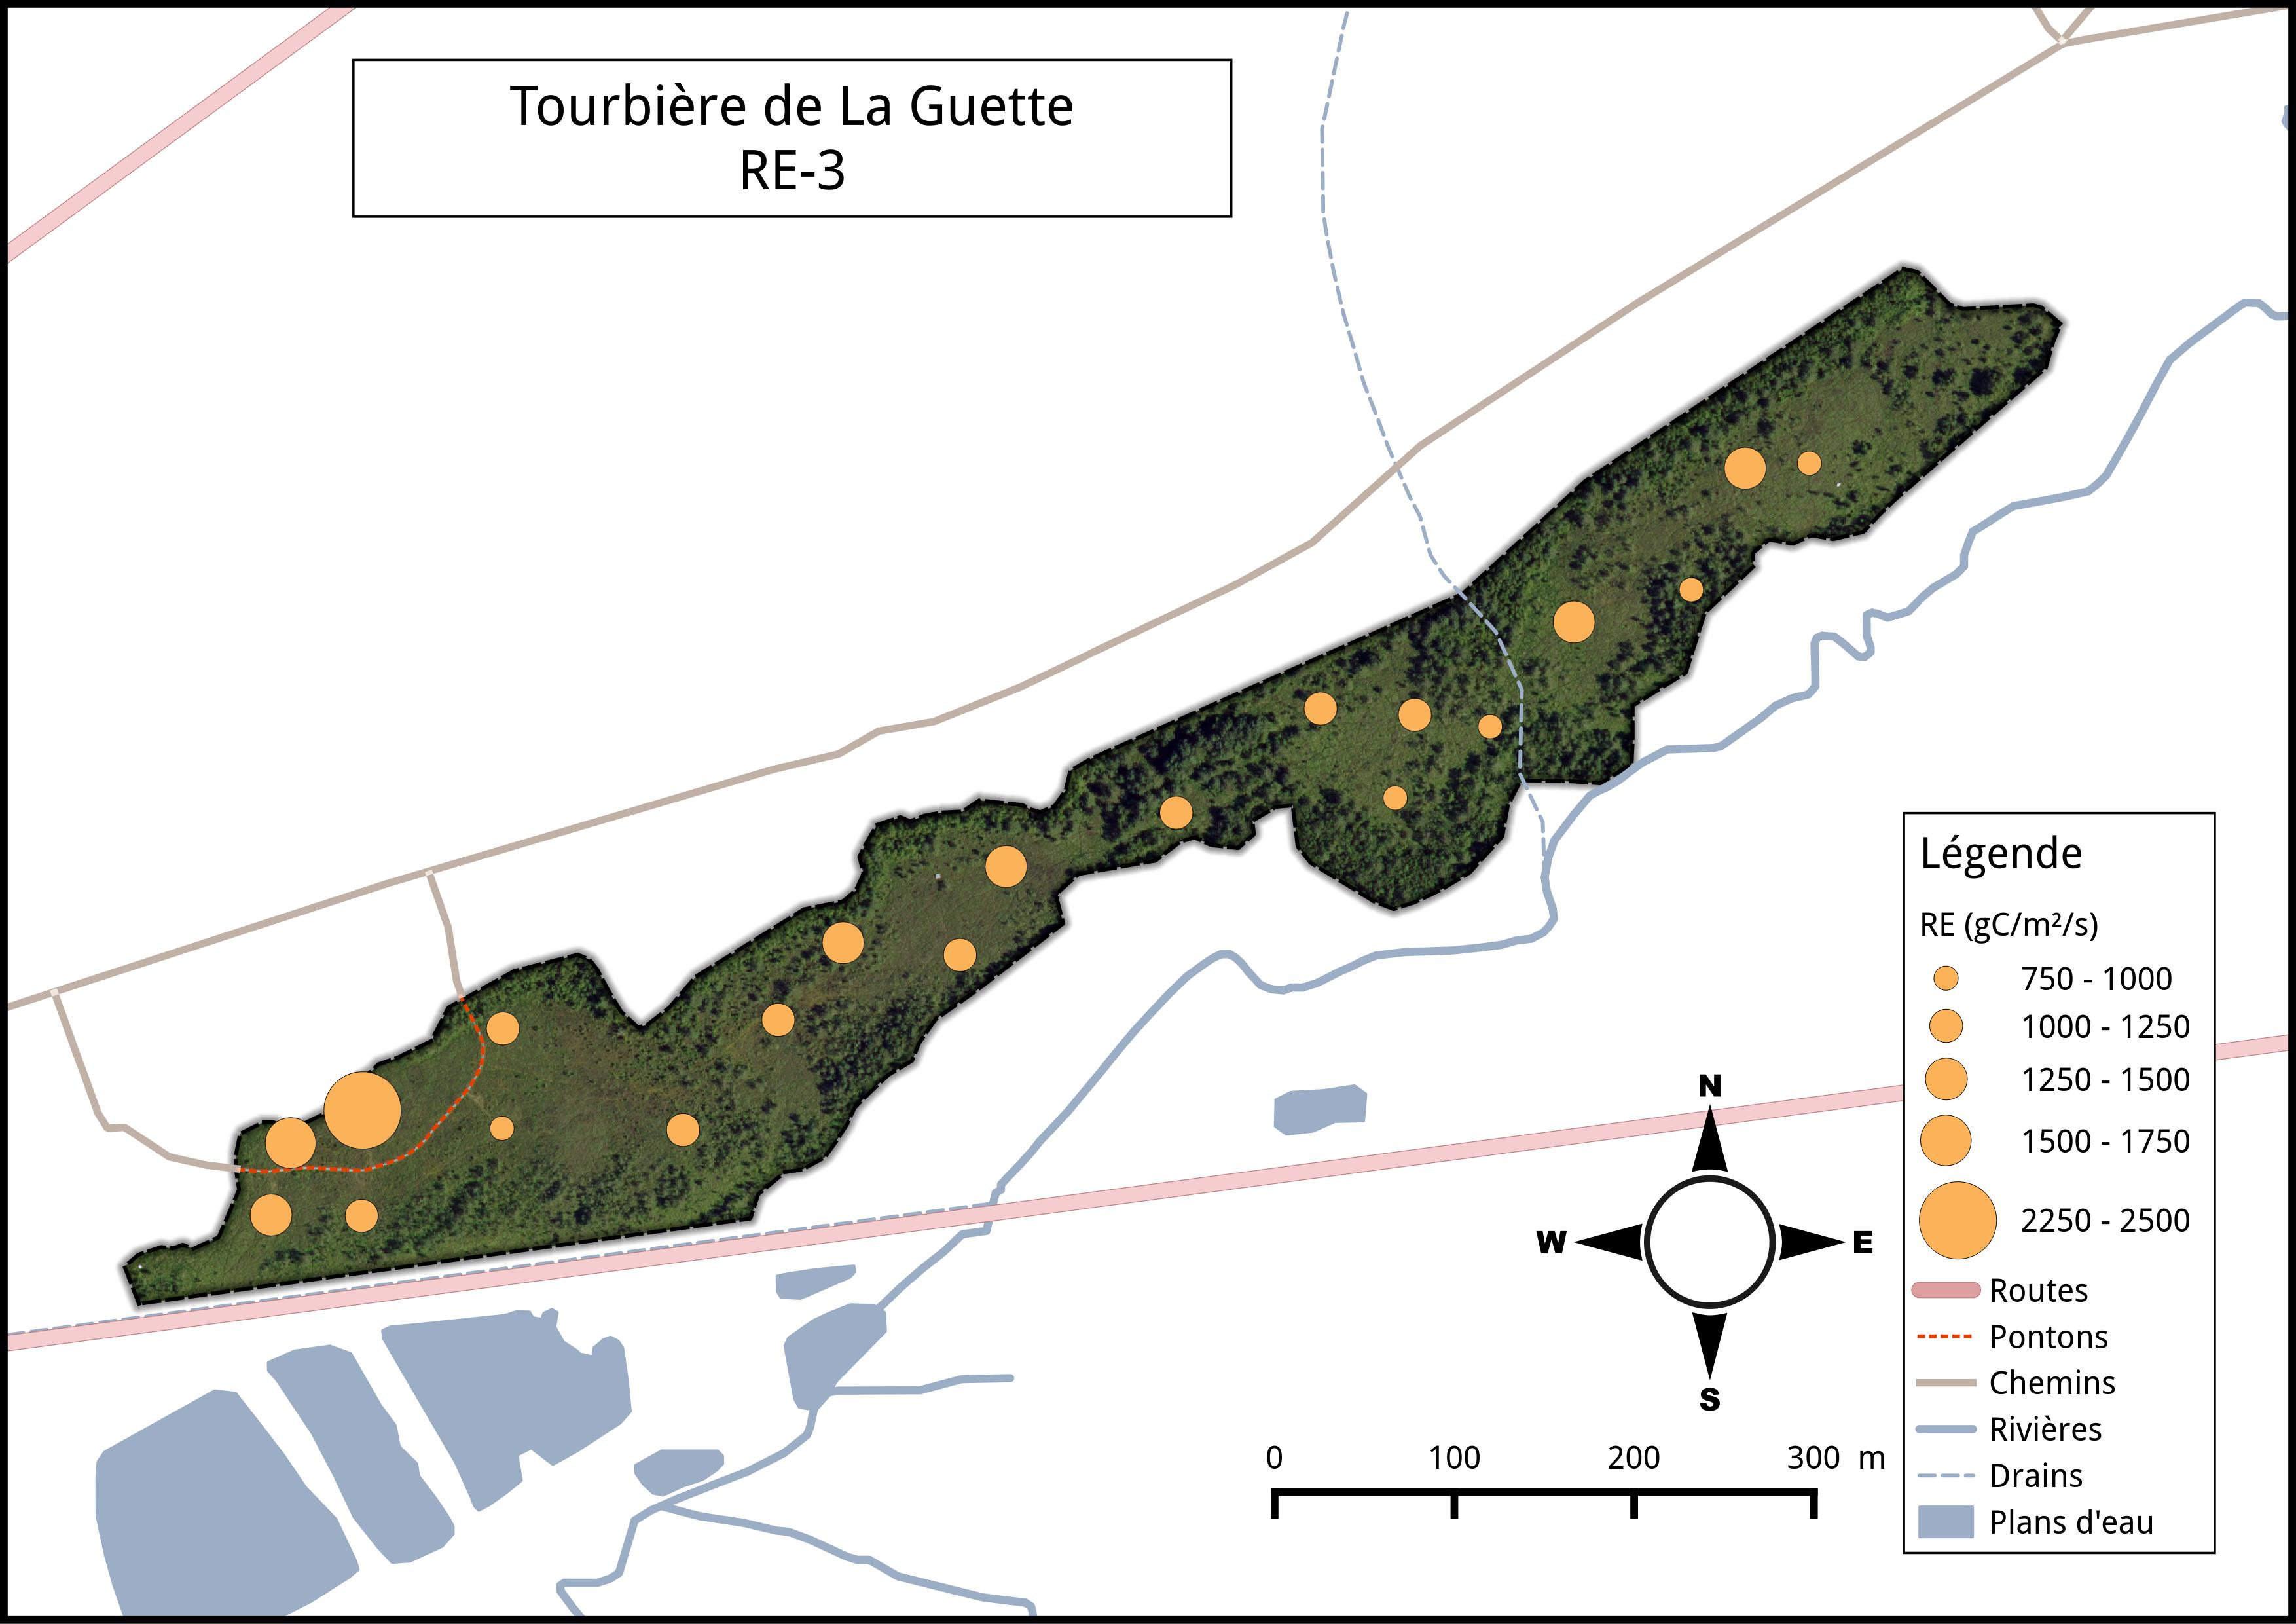
\includegraphics[width=.9\textwidth]{annexes/carte_RE-3}
\caption{Répartition de RE sur la tourbière de La Guette en \si{\gcma} à partir du modèle RE-3}
\label{fig:rep_RE-3}
\end{figure}


%\subsection{RE-3}
%
%\begin{figure}[!hbt]
%\centering
%
%\end{figure}




\clearpage
\section{Tableau modélisation par groupe de végétation}
\label{sec:mdl_grp_veg}

%\begin{table}
%\centering
%\caption{Valeur des paramètres des équations utilisées pour modéliser les flux et sensibilité relative (en \%) des flux en réponse à une variation de $\pm$\SI{10}{\percent} de chacun des paramètres des modèles.}
%\label{table:mdl_par_grp_veg}
%\hspace*{-1cm}
%\begin{tabular}{llcccccccccccc}\toprule
%\multicolumn{2}{l}{Groupe :} & \multicolumn{3}{c}{Mousse} & \multicolumn{3}{c}{Mix} & \multicolumn{3}{c}{Herbe} & \multicolumn{3}{c}{Arbuste}\\
%& par & valeur & se & pval & valeur & se & pval & valeur & se & pval & valeur & se & pval  \\ \midrule
%\multicolumn{14}{l}{PPB-1 -- équations~\ref{eq:juneTair} et \ref{eq:PPB_bubier}}  \\ [+.5ex]
%& a & 11.22 & 17.48 & 0.000 & 1155 & 2998 & 0.974 & 80.90 & 930 & 0.916 & 18.74 & 312 & 0.753 \\
%& b & 33.09 & 17.01 & 0.000 & 167 & 521 & 0.850  & 72.30 & 283.52 & 0.729 & 54.21 & 185 & 0.597 \\
%& c & 14.56 & 37.24 & 0.016 & 64.49 & 304.6 & 0.747 & 32.24 & 164.12 & 0.551 & 31.05 & 164 & 0.551\\
%%& i &  1.84 & 21.6  & 0.93 \\[+1ex]
%\multicolumn{14}{l}{PPB-2 -- équations~\ref{eq:juneTairIV} et \ref{eq:PPB_bubier}}  \\ [+.5ex]
%& a & 16.74 & 49.53 & 0.062 & 42.91 &  70.19 & 0.175 & 38.57 & 31.68 & 0.007 & 23.96 & 33.90 & 0.010\\
%& b & 31.87 & 14.40 & 0.000 & 51.49 &  47.42 & 0.052 & 35.69 & 38.50 & 0.021 & 33.27 & 47.74 & 0.054\\
%& c & 14.60 & 34.89 & 0.012 & 30.34 &  43.26 & 0.035 & 21.99 & 60.90 & 0.123 & 23.57 & 70.42 & 0.176\\
%& d &  2.12 & 202.8 & 0.629 & -1.83 & 256.27 & 0.702 &  0.10 &  2123 & 0.963 &  0.27 & 910.8 & 0.914\\
%%& i &  1.84 & 21.6  & 0.93 \\[+1ex]
%\multicolumn{14}{l}{RE-1 -- équation~\ref{eq:RE_T}}  \\ [+.5ex]
%& a & 0.23 & 19.90 & 0.48 & 18.80 & 0.000 & 0.32 & 41.44 & \\
%& b & 0.11 &  6.47 & 0.09 &  7.11 & 0.000 & 0.11 \\[+1ex]
%\multicolumn{14}{l}{RE-3 -- équation~\ref{eq:RE_TH}}  \\ [+.5ex]
%& a & 0 & 0 & 0.01 \\
%& b & 0.08 & 0.01 & \\
%& c & 0.33 & 0.06 & 0 \\[+1ex]
%\bottomrule
%\end{tabular}
%\hspace*{-1cm}
%\end{table}

\begin{table}
\centering
\caption{Valeur des paramètres des équations utilisées pour modéliser les flux de RE par groupe de végétation avec se l'erreur standard (en \si{\percent}) et pval la p-value.}
\label{table:mdl_par_grp_veg_er}
\hspace*{-1cm}
\begin{tabular}{lccccccccc}\toprule
%\multicolumn{2}{l}{Groupe :} & \multicolumn{3}{c}{Mousse} & \multicolumn{3}{c}{Mix} & \multicolumn{3}{c}{Herbe} & \multicolumn{3}{c}{Arbuste}\\
 & \multicolumn{3}{l}{a} & \multicolumn{3}{l}{b} & \multicolumn{3}{l}{c} \\  \cmidrule(lr){2-4} \cmidrule(lr){5-7} \cmidrule(lr){8-10}
Groupe & valeur & se & pval & valeur & se & pval & valeur & se & pval \\ \midrule
\multicolumn{10}{l}{RE-1 -- équation~\ref{eq:RE_T}}  \\ [+.5ex]
Mousse  & 0.23 & 19.90 & 0.000 & 0.11 &  6.47 & 0.000 & & & \\
Mixe    & 0.48 & 18.80 & 0.000 & 0.09 &  7.11 & 0.000 & & & \\
Herbe   & 0.32 & 41.44 & 0.027 & 0.11 & 13.47 & 0.000 & & & \\
Arbuste & 0.50 & 26.02 & 0.001 & 0.09 & 11.10 & 0.000 & & & \\
\multicolumn{10}{l}{RE-3 -- équation~\ref{eq:RE_TH}}  \\ [+.5ex]
Mousse  & 0.00 &  38.47 & 0.019 & 0.08 &  8.32 & 0.000 & 0.27 & 15.28 & 0.000 \\ 
Mixe    & 0.00 & 219.38 & 0.654 & 0.09 &  7.93 & 0.000 & 0.49 & 19.16 & 0.000 \\
Herbe   & 0.01 &  48.37 & 0.054 & 0.08 & 14.79 & 0.000 & 0.26 & 42.80 & 0.032 \\
Arbuste & 0.01 &  34.85 & 0.011 & 0.07 & 11.09 & 0.000 & 0.47 & 19.93 & 0.000 \\
\bottomrule
\end{tabular}
\hspace*{-1cm}
\end{table}

%\begin{table}
\begin{sidewaystable}
\centering
\caption{Valeur des paramètres des équations utilisées pour modéliser les flux de PPB par groupe de végétation avec se l'erreur standard (en \si{\percent}) et pval la p-value.}
\label{table:mdl_par_grp_veg_gpp}
%\hspace*{-1cm}
\begin{tabular}{lcccccccccccc}\toprule
%\multicolumn{2}{l}{Groupe :} & \multicolumn{3}{c}{Mousse} & \multicolumn{3}{c}{Mix} & \multicolumn{3}{c}{Herbe} & \multicolumn{3}{c}{Arbuste}\\
 & \multicolumn{3}{l}{a} & \multicolumn{3}{l}{b} & \multicolumn{3}{l}{c} & \multicolumn{3}{l}{d} \\ \cmidrule(lr){2-4} \cmidrule(lr){5-7} \cmidrule(lr){8-10} \cmidrule(lr){11-13}
Groupe & valeur & se & pval & valeur & se & pval & valeur & se & pval & valeur & se & pval \\ \midrule
\multicolumn{13}{l}{PPB-1 -- équations~\ref{eq:juneTair} et \ref{eq:PPB_bubier}}  \\ [+.5ex]
Mousse & 11.22 & 17.48 & 0.000 & 33.09 & 17.01 & 0.000 & 14.56 & 37.24 & 0.016 &   &  &  \\
Mix & 1154.99 & 2997.91 & 0.974 & 167.22 & 521.44 & 0.850 & 64.49 & 304.55 & 0.747 &   &  &  \\
Herbe & 80.90 & 930.16 & 0.916 & 72.30 & 283.52 & 0.729 & 32.24 & 216.07 & 0.650 &   &   &  \\ 
Arbuste & 18.74 & 312.12 & 0.753 & 54.21 & 185.21 & 0.597 & 31.05 & 164.12 & 0.551 &   &   &  \\ [+1ex]
\multicolumn{13}{l}{PPB-2 -- équations~\ref{eq:juneTairIV} et \ref{eq:PPB_bubier}}  \\ [+.5ex]
Mousse & 16.74 & 49.53 & 0.062 & 31.87 & 14.40 & 0.000 & 14.60 & 34.89 & 0.012 & 2.12 & 202.80 & 0.629 \\ 
Mix & 42.91 & 70.19 & 0.175 & 51.49 & 47.42 & 0.052 & 30.34 & 43.26 & 0.035 & -1.83 & -256.27 & 0.702 \\ 
Herbe & 38.57 & 31.68 & 0.007 & 35.69 & 38.50 & 0.021 & 21.99 & 60.90 & 0.123 & 0.10 & 2122.54 & 0.963 \\
Arbuste & 23.96 & 33.90 & 0.010 & 33.27 & 47.74 & 0.054 & 23.57 & 70.42 & 0.176 & 0.27 & 910.80 & 0.914 \\
\bottomrule
\end{tabular}
%\hspace*{-1cm}
\end{sidewaystable}
%\end{table}


\clearpage
\newgeometry{includeheadfoot, hmargin=10mm, vmargin=15mm, bindingoffset=0.5cm}
\section{Tableau de données bibliographiques}
\label{sec:bibliodata}

%\begin{minipage}{\textwidth}

%\begin{landscape}
%\begin{sidewaystable}
%\begin{table}
\scriptsize
\setlength{\tabcolsep}{2pt}
\begin{longtable}{llllllllllllll}
%\footnotesize
%\centering
\caption{ Références et données utilisés. La colonne « Année » se réfère aux années de mesure, les flux (ENE, RE, PPB, \chh, COD, BCNE) sont exprimés en \si{\gcma}. La colonne « Classif » décrit le type de tourbière (Haut-marais : bog ou Bas-marais : fen). La colonne « Manag. » décrit une éventuelle utilisation du site. Les colonnes « TMA » et « PMA » correspondent respectivement aux températures moyennes annuelles et aux précipitation moyennes annuelles. Les latitudes et longitudes (colonne « Lat/Lon ») sont exprimés en degrés décimaux}\\
\label{table:bibliodata}\\
%\vspace*{-1cm}\\
%\begin{tabular}{cccccccccccccccc}
\toprule
Année & ENE & RE & PPB & \chh & COD & BCNE & Flux considérés & Classif. & Manag. & TMA & PMA & Lat/Lon & Référence \\ \midrule
1993 & 97,3 & 53,9 & 151,2 & 6,05 & 43,8 & 34,2 & \coo, \chh, COD & bog & natural & 5,2 & 1953 & 54,69 ; -2,38 & \citealp{worrall2009}\\
1994 & 120,7 & 52,1 & 172,8 & 6,05 & 22,9 & 61,1 &  &  &  &  &   &  &  \\
1995 & 133,2 & 54,8 & 188 & 6,05 & 26,3 & 75,8 &  &  &  &  &   &  &  \\
1996 & 129,9 & 49,4 & 179,3 & 6,05 & 19,6 & 83,2 &  &  &  &  &  &  & \\
1997 & 126,7 & 54,8 & 181,5 & 6,05 & 24,9 & 66 &  &  &  &  &  &   & \\
1998 & 111,2 & 53 & 164,2 & 6,05 & 66,1 & 9,8 &  &  &  &  &  &   & \\
1999 & 123,3 & 53,9 & 177,2 & 6,05 & 12,1 & 83,2 &  &  &  &  &   &  &\\ 
2000 & 125,1 & 52,1 & 177,2 & 6,05 & 39,1 & 58,7 &  &  &  &  &   &  & \\
2001 & 125,8 & 55,7 & 181,5 & 6,05 & 86,3 & 17,1 &  &  &  &  &   &  & \\
2002 & 115,3 & 57,5 & 172,8 & 6,05 & 56,6 & 26,9 &  &  &  &  &   &  & \\
2003 & 118,4 & 56,6 & 175 & 6,05 & 24,9 & 80,7 &  &  &  &  &  &   & \\
2004 & 123,8 & 51,2 & 175 & 6,05 & 67,4 & 24,5 &  &  &  &  &  &   & \\
2005 & 131,7 & 58,4 & 190,1 & 6,05 & 31,7 & 75,8 &  &  &  &  &   &  & \\ [+1.5ex]
1999 & 60,5 &    &    & 2,9 & 11,5 & 44,7 & \coo, \chh, COD & bog & natural & 6,0 & 943 & 45,4 ; -75,48 & \citealp{roulet2007}\\
2000 & 34,6 &    &    & 4,3 & 13 & 17,3 &  &  &  &  &  &  & \\
2001 & 2 &    &    & 2,9 & 11,5 & -14,4 &  &  &  &  &  &  & \\
2002 & 20,2 &    &    & 2,9 & 17,3 & -0,3 &  &  &  &  & &  & \\
2003 & 14,4 &    &    & 3,2 & 17,3 & -5,8 &  &  &  &  & &  & \\
2004 & 112,4 &    &    & 3,5 & 18,7 & 89,4 &  &  &  &  & &  & \\ [+1.5ex]
2004 & 55 &    &    & 9 & 20,4 & 27 & \coo, \chh, COD & fen & natural & 1,2 & 523 & 64,1 ; 19,33 & \citealp{nilsson2008}\\
2005 & 48 &    &    & 14 & 15,1 & 20 &  &  &  &  &  &   &  \\ [+1.5ex]
2004 & 137,5 & 241,5 & 379 & 1,5 &    & 134 & \coo, \chh, COD & bog & natural & 6,6 & 1417 & 47,2 ; 6,79 & \citealp{bortoluzzi2006a}\\
2005 & 155,5 & 286,5 & 442 & 1,6 &    & 152,5 &  &  &  &  &  &  & \\ [+1.5ex]
2010 & -244,1 &    &    & 6,6 &    & -250,7 & \coo, \chh, COD & bog & natural & 5,2 & 996 & 48,0 ; -69,43 & \citealp{strack2013}\\ [+1.5ex]
2003 & 66,8 &    &    & 3,8 & 13,5 & 49,6 & \coo, \chh, COD &  bog & natural & 10,6 & 2500 & 51,6 ; -9,55 & \citealp{koehler2011}\\
2004 & 67,2 &    &    & 3,6 & 13,1 & 50,5 &  &  &   &  & 2500 &  &  \\
2005 & 84 &    &    & 4,7 & 13,9 & 65,6 &  &  &   &  & 2500 &  &  \\
2006 & 12,5 &    &    & 4,6 & 16,5 & -8,6 &  &  &  &  & 2952 &   & \\
2007 & 13,5 &    &    & 4,2 & 11,9 & -2,8 &  &  &  &  & 2235 &   & \\
2008 & 42,7 &    &    & 3,6 & 15,0 & 24,1 &  &  &  &  & 2500 &   & \\ [+1.5ex]
2007 & 136 &    &    & 0,29 & 17,34 & 101 & \coo, \chh, COD  & bog & grazing & 10 & 1155 & 55,8 ; -3,24 & \citealp{dinsmore2010}\\
2008 & 93,5 &    &    & 0,35 & 30,75 & 38,2 &  &  &  &  &  &  &    \\ [+1.5ex]
2001 & 70 & 500 & 570 & 5 & 5 & 60 & \coo, \chh, COD & bog & natural & 6,0 & 943 & 45,4 ; -75,48 & \citealp{moore2002}\\ [+1.5ex]
1992 & 10,3 & 153,4 & 163,7 & 4,1 & 4,2 & 2 & \coo, \chh, COD & bog & natural &    &    & 63,7 ; 20,10 & \citealp{waddington2000}\\
1993 & 3 & 196,5 & 199,5 & 3,9 & 6,7 & -7,6 &  &  &  &  &  &  & \\ [+1.5ex]
2004 & 51,3 &    &    &    &    & -31,9 & \coo, \chh, COD & fen & natural & 3,3 & 713 & 61,8 ; 24,20 & \citealp{aurela2007}\\
2005 & 59,7 &    &    &    &    & -40,3 &  &  &  &  &  &  & \\ [+1.5ex]
1994 & -145 &    &    &    &    & -145 & \coo, \chh, COD & fen & natural & 8,2 & 1071 & 43,2 ; -71,06 & \citealp{carroll1997}\\ [+1.5ex]
2010 & 75,8 & 759,5 & 835,3 & 0,05 &    & 75,8 & \coo, \chh & bog & natural & 8,6 & 795 & 53,0 ; 7,32 & \citealp{beyer2015a}\\
2010 & 201,7 & 856,3 & 1058 & 16,2 &    & 185,5 &  & bog &  &  &  &  &  \\
2010 & 113,6 & 420,3 & 533,9 & 22,4 &    & 91,2 &  & bog &  &  &  &  &  \\
2011 & -9,2 & 997,3 & 988,1 & 0,11 &    & -9,3 &  & bog &  &  &  &  &  \\
2011 & -29,7 & 1052,2 & 1022,5 & 20,2 &    & -49,9 &  & bog &  &  &  &  & \\
2011 & 76,2 & 584,5 & 660,7 & 24,2 &    & 52 &  & bog &  &  &  &  & \\ [+1.5ex]
2008 & -142 & 2180 &    &    &    & -142 & \coo, \chh & fen & grassland & 8,9 & 695 & 52,3 ; 8,20 & \citealp{beyer2015}\\
2009 & -565 & 2125 &    &    &    & -565 &  &  &  &  &  &  &  \\
2010 & -293 & 2010 &    &    &    & -293 &  &  &  &  &  &  &  \\
2011 & -245 & 2439 &    &    &    & -245 &  &  &  &  &  &  &  \\ [+1.5ex]
2011 & -84 & & & 17 & & -102 & \coo, \chh & bog & natural & 9,6 & 821 & 53,7 ; -9,8 & \citealp{vanselow-algan2015}\\
2011 & -16 & & & 27 & & -44 & & &  & 9,6 & 821 & 53,7 ; -9,8 &\\
2011 & -67 & & & 40 & & -395 & &  & & 9,6 & 821 & 53,7 ; -9,8 &\\ [+1.5ex]
2009 & -390 & 2894 & 2512 &    &    & -390 & \coo & fen & grassland & 9,6 & 913 & 55,9 ; 8,43 & \citealp{elsgaard2012}\\
2009 & -450 & 2539 & 2102 &    &    & -450 & \coo & fen & grassland & 9,0 & 579 & 56,4 ; 10,40 & \\
2009 & -690 & 2839 & 2157 &    &    & -690 & \coo & bog & grassland & 8,6 & 702 & 57,2 ; 9,83 & \\ [+1.5ex]
2004 & 144 &    &    &    &    & 144 & \coo & fen & natural & 2,1 & 504 & 55,0 ; -112,47 & \citealp{syed2006}\\ [+1.5ex]
1997 & 20 &    &    &    &    & 20 & \coo & fen & naturel & -9,2 & 214 & 74,5 ; -20,57 & \citealp{nordstroem2001}\\ [+1.5ex]
2008 & 61,98 &    &    &    & 3,56 & 55,77 & \coo & fen & natural & -0,2 & 321 & 68,4 ; 19,05 & \citealp{olefeldt2012}\\
2009 & 38,42 &    &    &    & 2,76 & 33,01 &  &  &   & -0,4 & 281 &  &  \\  [+1.5ex]
2009 & -404,1 & 858,2 & 454,1 &    &    & -101,2 & \coo  & fen & natural & -4,28 & 738 & 54,1 ; 72,50 & \citealp{trudeau2014}\\
2010 & -272,4 & 755,6 & 483,2 &    &    & -71,3 & \coo &   &  &  &  &  & \\ [+1.5ex]
2001 & 58 & 261 & 319 &    &    & 58 & \coo & fen & natural & 1,8 & 888 & 64,2 ; 19,55 & \citealp{peichl2014}\\
2002 & 60 & 443 & 503 &    &    & 60 &  &  &  & 2,9 & 533 &  &  \\
2003 & 47 & 402 & 449 &    &    & 47 &  &  &  & 2,3 & 584 &  &  \\
2004 & 59 & 298 & 358 &    &    & 59 &  &  &  & 0,9 & 650 &  &  \\
2005 & 58 & 322 & 380 &    &    & 58 &  &  &  & 3,1 & 659 &  &  \\
2006 & 18 & 265 & 283 &    &    & 18 &  &  &  & 2,8 & 661 &  &  \\
2007 & 48 & 254 & 302 &    &    & 48 &  &  &  & 2,8 & 586 &  &  \\
2008 & 105 & 351 & 456 &    &    & 105 &  &  &  & 2,0 & 751 &  & \\
2009 & 41 & 174 & 215 &    &    & 41 &  &  &  & 0,4 & 702 &  &  \\
2010 & 66 & 137 & 203 &    &    & 66 &  &  &  & 3,5 & 639 &  &  \\
2011 & 79 & 261 & 340 &    &    & 79 &  &  &  & 1,9 & 707 &  &  \\
2012 & 57 & 172 & 229 &    &    & 57 &  &  &  & 2,3 & 630 &  &  \\ [+1.5ex]
1997 & 4 &    &    &    &    & 4 & \coo & fen & natural & -1 & 470 & 69,1 ; 27,28 & \citealp{aurela2004}\\
1998 & 21 &    &    &    &    & 21 &  &   &  &  &  &  & \\
1999 & 8 &    &    &    &    & 8 &  &  &   &  &  &  &  \\
2000 & 6 &    &    &    &    & 6 &  &  &   &  &  &  &  \\
2001 & 37 &    &    &    &    & 37 &  &   &  &  &  &  & \\
2002 & 53 &    &    &    &    & 53 &  &   &  &  &  &  & \\ [+1.5ex]
2008 & -668 & 3518 & 2359 &    &    & -668 & \coo & fen & grassland & 9,5 & 913 & 55,9 ; 8,4 & \citealp{gorres2014}\\
2008 & -736 & 2836 & 2100 &    &    & -736 &  & fen & grassland & 9,1 & 579 & 56,4 ; 10,4 &  \\
2008 & -614 & 2727 & 2114 &    &    & -614 &  & bog & grassland & 8,8 & 702 & 57,1 ; 9,8 &  \\
\bottomrule
%\end{tabular}
%\hspace*{-1cm}
%\end{table}
\end{longtable}
%\end{sidewaystable}
%\end{landscape}

%\end{minipage}



%Année & ENE & RE & PPB & \chh & COD & BCNE & Flux considérés & Site(s) & Classif. & Manag. & TMA & PMA & Lat/Lon & Référence \\ \midrule
%1993 & 97,3 & 53,9 & 151,2 & 6,05 & 43,8 & 34,2 & \coo, \chh, COD & Trout Beck & bog & natural & 5,2 & 1953 & 54,69 ; -2,38 & \citealp{worrall2009}\\
%1994 & 120,7 & 52,1 & 172,8 & 6,05 & 22,9 & 61,1 &  &  &  &  &  &  &  &  \\
%1995 & 133,2 & 54,8 & 188 & 6,05 & 26,3 & 75,8 &  &  &  &  &  &  &  &  \\
%1996 & 129,9 & 49,4 & 179,3 & 6,05 & 19,6 & 83,2 &  &  &  &  &  &  &  & \\
%1997 & 126,7 & 54,8 & 181,5 & 6,05 & 24,9 & 66 &  &  &  &  &  &  &   & \\
%1998 & 111,2 & 53 & 164,2 & 6,05 & 66,1 & 9,8 &  &  &  &  &  &  &   & \\
%1999 & 123,3 & 53,9 & 177,2 & 6,05 & 12,1 & 83,2 &  &  &  &  &  &   &  &\\ 
%2000 & 125,1 & 52,1 & 177,2 & 6,05 & 39,1 & 58,7 &  &  &  &  &  &   &  & \\
%2001 & 125,8 & 55,7 & 181,5 & 6,05 & 86,3 & 17,1 &  &  &  &  &  &   &  & \\
%2002 & 115,3 & 57,5 & 172,8 & 6,05 & 56,6 & 26,9 &  &  &  &  &  &   &  & \\
%2003 & 118,4 & 56,6 & 175 & 6,05 & 24,9 & 80,7 &  &  &  &  &  &  &   & \\
%2004 & 123,8 & 51,2 & 175 & 6,05 & 67,4 & 24,5 &  &  &  &  &  &  &   & \\
%2005 & 131,7 & 58,4 & 190,1 & 6,05 & 31,7 & 75,8 &  &  &  &  &  &   &  & \\ [+1ex]
%1999 & 60,5 & NA & NA & 2,9 & 11,5 & 44,7 & \coo, \chh, COD & Mer Bleue & bog & natural & 6,0 & 943 & 45,4 ; -75,48 & \citealp{roulet2007}\\
%2000 & 34,6 & NA & NA & 4,3 & 13 & 17,3 &  &  &  &  &  &    &  & \\
%2001 & 2 & NA & NA & 2,9 & 11,5 & -14,4 &  &  &  &  &  &   &  & \\
%2002 & 20,2 & NA & NA & 2,9 & 17,3 & -0,3 &  &  &  &  &  &  &  & \\
%2003 & 14,4 & NA & NA & 3,2 & 17,3 & -5,8 &  &  &  &  &  &  &  & \\
%2004 & 112,4 & NA & NA & 3,5 & 18,7 & 89,4 &  &  &  &  &  &  &  & \\ [+1ex]
%2004 & 55 & NA & NA & 9 & 20,4 & 27 & \coo, \chh, COD & Degero Stormyr & fen & natural & 1,2 & 523 & 64,1 ; 19,33 & \citealp{nilsson2008}\\
%2005 & 48 & NA & NA & 14 & 15,1 & 20 &  &  &  &  &  &  &  &  \\ [+1ex]
%2004 & 137,5 & 241,5 & 379 & 1,5 & NA & 134 & \coo, \chh, COD & Sur les Seignes & bog & natural & 6,6 & 1417 & 47,2 ; 6,79 & \citealp{bortoluzzi2006a}\\
%2005 & 155,5 & 286,5 & 442 & 1,6 & NA & 152,5 &  &  &  &  &  &  &  & \\ [+1ex]
%2010 & -244,1 & NA & NA & 6,6 & NA & -250,7 & \coo, \chh, COD & Bois-des-Bel & bog & natural & 5,2 & 996 & 48,0 ; -69,43 & \citealp{strack2013}\\ [+1ex]
%2003 & 66,8 & NA & NA & 3,8 & 13,5 & 49,6 & \coo, \chh, COD & NA & bog & natural & 10,6 & 2500 & 51,6 ; -9,55 & \citealp{koehler2011}\\
%2004 & 67,2 & NA & NA & 3,6 & 13,1 & 50,5 &  &  &  &  &  & 2500 &  &  \\
%2005 & 84 & NA & NA & 4,7 & 13,9 & 65,6 &  &  &  &  &  & 2500 &  &  \\
%2006 & 12,5 & NA & NA & 4,6 & 16,5 & -8,6 &  &  &  &  &  & 2952 &   & \\
%2007 & 13,5 & NA & NA & 4,2 & 11,9 & -2,8 &  &  &  &  &  & 2235 &   & \\
%2008 & 42,7 & NA & NA & 3,6 & 15,0 & 24,1 &  &  &  &  &  & 2500 &   & \\ [+1ex]
%2007 & 136 & NA & NA & 0,29 & 17,34 & 101 & \coo, \chh, COD & Auchencorth & bog & grazing & 10 & 1155 & 55,8 ; -3,24 & \citealp{dinsmore2010}\\
%2008 & 93,5 & NA & NA & 0,35 & 30,75 & 38,2 &  &  &  &  &  &  &  &   \\ [+1ex]
%2001 & 70 & 500 & 570 & 5 & 5 & 60 & \coo, \chh, COD & Mer Bleue & bog & natural & 6,0 & 943 & 45,4 ; -75,48 & \citealp{moore2002}\\ [+1ex]
%1992 & 10,3 & 153,4 & 163,7 & 4,1 & 4,2 & 2 & \coo, \chh, COD & Stor-amyran & bog & natural & NA & NA & 63,7 ; 20,10 & \citealp{waddington2000}\\
%1993 & 3 & 196,5 & 199,5 & 3,9 & 6,7 & -7,6 &  &  &  &  &  &  &  &  \\ [+1ex]
%2004 & 51,3 & NA & NA & NA & NA & -31,9 & \coo, \chh, COD & Siikaneva & fen & natural & 3,3 & 713 & 61,8 ; 24,20 & \citealp{aurela2007}\\
%2005 & 59,7 & NA & NA & NA & NA & -40,3 &  &  &  &  &  &  &  & \\ [+1ex]
%1994 & -145 & NA & NA & NA & NA & -145 & \coo, \chh, COD & Sallie's Fen & fen & natural & 8,2 & 1071 & 43,2 ; -71,06 & \citealp{carroll1997}\\ [+1ex]
%2010 & 75,8 & 759,5 & 835,3 & 0,05 & NA & 75,8 & \coo, \chh & leegmoor molinia & bog & natural & 8,6 & 795 & 53,0 ; 7,32 & \citealp{beyer2015a}\\
%2010 & 201,7 & 856,3 & 1058 & 16,2 & NA & 185,5 &  & leegmoor eriophorum & bog &  &  &  &  &  \\
%2010 & 113,6 & 420,3 & 533,9 & 22,4 & NA & 91,2 &  & leegmoor sphagnum & bog &  &  &  &  &  \\
%2011 & -9,2 & 997,3 & 988,1 & 0,11 & NA & -9,3 &  & leegmoor molinia & bog &  &  &  &  &  \\
%2011 & -29,7 & 1052,2 & 1022,5 & 20,2 & NA & -49,9 &  & leegmoor eriophorum & bog &  &  &  &  & \\
%2011 & 76,2 & 584,5 & 660,7 & 24,2 & NA & 52 &  & leegmoor sphagnum & bog &  &  &  &  & \\ [+1ex]
%2008 & -142 & 2180 & NA & NA & NA & -142 & \coo, \chh & Dümmer peatland & fen & grassland & 8,9 & 695 & 52,3 ; 8,20 & \citealp{beyer2015}\\
%2009 & -565 & 2125 & NA & NA & NA & -565 &  &  &  &  &  &  &  &  \\
%2010 & -293 & 2010 & NA & NA & NA & -293 &  &  &  &  &  &  &  &  \\
%2011 & -245 & 2439 & NA & NA & NA & -245 &  &  &  &  &  &  &  &  \\ [+1ex]
%2009 & -390 & 2894 & 2512 & NA & NA & -390 & \coo & W-PG & fen & grassland & 9,6 & 913 & 55,9 ; 8,43 & \citealp{elsgaard2012}\\
%2009 & -450 & 2539 & 2102 & NA & NA & -450 & \coo & E-PG & fen & grassland & 9,0 & 579 & 56,4 ; 10,40 & \\
%2009 & -690 & 2839 & 2157 & NA & NA & -690 & \coo & N-PG & bog & grassland & 8,6 & 702 & 57,2 ; 9,83 & \\ [+1ex]
%2004 & 144 & NA & NA & NA & NA & 144 & \coo & NA & fen & natural & 2,1 & 504 & 55,0 ; -112,47 & \citealp{syed2006}\\ [+1ex]
%1997 & 20 & NA & NA & NA & NA & 20 & \coo & Zackenberg & fen & naturel & -9,2 & 214 & 74,5 ; -20,57 & \citealp{nordstroem2001}\\ [+1ex]
%2008 & 61,98 & NA & NA & NA & 3,56 & 55,77 & \coo & Stordalen & fen & natural & -0,2 & 321 & 68,4 ; 19,05 & \citealp{olefeldt2012}\\
%2009 & 38,42 & NA & NA & NA & 2,76 & 33,01 &  &  &  &  & -0,4 & 281 &  &  \\  [+1ex]
%2009 & -404,1 & 858,2 & 454,1 & NA & NA & -101,2 & \coo & Abeille & fen & natural & -4,28 & 738 & 54,1 ; 72,50 & \citealp{trudeau2014}\\
%2010 & -272,4 & 755,6 & 483,2 & NA & NA & -71,3 & \coo &  &  &  &  &  &  & \\ [+1ex]
%2001 & 58 & 261 & 319 & NA & NA & 58 & \coo & Degero Stormyr & fen & natural & 1,8 & 888 & 64,2 ; 19,55 & \citealp{peichl2014}\\
%2002 & 60 & 443 & 503 & NA & NA & 60 &  &  &  &  & 2,9 & 533 &  &  \\
%2003 & 47 & 402 & 449 & NA & NA & 47 &  &  &  &  & 2,3 & 584 &  &  \\
%2004 & 59 & 298 & 358 & NA & NA & 59 &  &  &  &  & 0,9 & 650 &  &  \\
%2005 & 58 & 322 & 380 & NA & NA & 58 &  &  &  &  & 3,1 & 659 &  &  \\
%2006 & 18 & 265 & 283 & NA & NA & 18 &  &  &  &  & 2,8 & 661 &  &  \\
%2007 & 48 & 254 & 302 & NA & NA & 48 &  &  &  &  & 2,8 & 586 &  &  \\
%2008 & 105 & 351 & 456 & NA & NA & 105 &  &  &  &  & 2,0 & 751 &  & \\
%2009 & 41 & 174 & 215 & NA & NA & 41 &  &  &  &  & 0,4 & 702 &  &  \\
%2010 & 66 & 137 & 203 & NA & NA & 66 &  &  &  &  & 3,5 & 639 &  &  \\
%2011 & 79 & 261 & 340 & NA & NA & 79 &  &  &  &  & 1,9 & 707 &  &  \\
%2012 & 57 & 172 & 229 & NA & NA & 57 &  &  &  &  & 2,3 & 630 &  &  \\ [+1ex]
%1997 & 4 & NA & NA & NA & NA & 4 & \coo & Kaamanen & fen & natural & -1 & 470 & 69,1 ; 27,28 & \citealp{aurela2004}\\
%1998 & 21 & NA & NA & NA & NA & 21 &  &  &  &  &  &  &  & \\
%1999 & 8 & NA & NA & NA & NA & 8 &  &  &  &  &  &  &  &  \\
%2000 & 6 & NA & NA & NA & NA & 6 &  &  &  &  &  &  &  &  \\
%2001 & 37 & NA & NA & NA & NA & 37 &  &  &  &  &  &  &  & \\
%2002 & 53 & NA & NA & NA & NA & 53 &  &  &  &  &  &  &  & \\ [+1ex]
%2008 & -668 & 3518 & 2359 & NA & NA & -668 & \coo & Western Jutland & fen & grassland & 9,5 & 913 & 55,9 ; 8,4 & \citealp{gorres2014}\\
%2008 & -736 & 2836 & 2100 & NA & NA & -736 &  & Eastern Jutland & fen & grassland & 9,1 & 579 & 56,4 ; 10,4 &  \\
%2008 & -614 & 2727 & 2114 & NA & NA & -614 &  & Northern Jutland & bog & grassland & 8,8 & 702 & 57,1 ; 9,8 &  \\


\restoregeometry